\documentclass[11pt, a4paper]{article}
\usepackage[utf8]{inputenc}
\usepackage[T1]{fontenc}
\usepackage{geometry}
\geometry{margin=1in} % Standard margins
\usepackage{graphicx} % For plots, diagrams, and LOGO
\usepackage{amsmath, amssymb, amsfonts} % Math symbols
\usepackage{booktabs} % Professional tables
\usepackage{hyperref} % Clickable links
\usepackage{algorithm} % For algorithms
\usepackage{algpseudocode} % For pseudocode
\usepackage{subcaption} % For side-by-side figures
\usepackage{listings} % For code snippets
\usepackage{xcolor} % For colors
\usepackage{csquotes} % For \enquote command
\usepackage{wrapfig}   % add this in your preamble
\usepackage{graphicx}
\usepackage{lipsum}
\setlength{\marginparwidth}{2cm}
\usepackage{todonotes}
\usepackage{epigraph}
\usepackage{tcolorbox}
\usepackage{fancyhdr}
\usepackage{placeins}
\pagestyle{fancy}
\fancyhf{} % clear default headers/footers
\fancyfoot[C]{\thepage} % add page number to center footer
\setlength{\headheight}{25.22153pt}
\addtolength{\topmargin}{-13.22153pt}
\usepackage{ragged2e}

\usepackage[backend=biber,style=ieee]{biblatex}
\addbibresource{ref.bib}

% --- Setup for Code Listings ---
\definecolor{codegray}{rgb}{0.5,0.5,0.5}
\definecolor{codepurple}{rgb}{0.58,0,0.82}
\lstset{ 
    language=Python,
    basicstyle=\ttfamily\small,
    commentstyle=\color{codegray},
    keywordstyle=\color{magenta},
    numberstyle=\tiny\color{codegray},
    numbers=left,
    frame=single,
    breaklines=true
}

% --- Hyperref Setup (Optional: removes red boxes around links) ---
\hypersetup{
    colorlinks=true,
    linkcolor=black,
    filecolor=magenta,      
    urlcolor=blue,
    citecolor=blue,
}


\renewcommand{\todo}[1]{\textcolor{red}{\textbf{TODO:} #1}}



\usepackage{listings}
\usepackage{xcolor}

% Define custom colors for the code
\definecolor{codegreen}{rgb}{0,0.6,0}
\definecolor{codegray}{rgb}{0.5,0.5,0.5}
\definecolor{codepurple}{rgb}{0.58,0,0.82}
\definecolor{backcolour}{rgb}{0.95,0.95,0.92}

% Setup the style
\lstdefinestyle{mystyle}{
    backgroundcolor=\color{backcolour},   
    commentstyle=\color{codegreen},
    keywordstyle=\color{magenta},
    numberstyle=\tiny\color{codegray},
    stringstyle=\color{codepurple},
    basicstyle=\ttfamily\footnotesize, % Small font for compactness
    breakatwhitespace=false,         
    breaklines=true,                 
    captionpos=b,                    
    keepspaces=true,                 
    numbers=left,                    
    numbersep=2pt,                  
    showspaces=false,                
    showstringspaces=false,
    showtabs=false,                  
    tabsize=1,
    frame=single % Adds a border
}

\lstset{style=mystyle}


\begin{document}


\begin{titlepage}
    \centering
    \vspace*{1cm}
    {\Large \textbf{Deep Reinforcement Learning for Steering Control\\of a Foiling Sailboat}}\\
\vspace{1.5cm}

   
    {\textbf{D. Dilruwan}\textsuperscript{1} \& \textbf{W. Peifeng}\textsuperscript{1}} \\
    \vspace{0.8cm}

    Supervised by \\
    {Benjamin Negrevergne\textsuperscript{2} \& Camille Negrevergne\textsuperscript{2}} \\
    
    \vspace{0.5cm}
    
    {\textsuperscript{1}\textit{ENSAI} \quad \textsuperscript{2}\href{https://nautia.fr/}{NAUTIA}} \\
    
    \vspace{0.5cm}
    
    {\footnotesize
     \texttt{\{peifeng.wang, dilruwan.dehiwalage-don\}@eleve.ensai.fr}\\[2pt]
     
    \texttt{\{camille, benjamin\}@nautia.fr}
    }
    
    \vfill
    {\large \today}
    
    \vspace{1cm}

    \raggedright
    
\includegraphics[width=8cm]{resources/logo/logo_nautia_ensai.pdf} 
\end{titlepage}


\thispagestyle{plain} 
\begin{abstract}
    \noindent  \large In the context of elite offshore racing, such as the Vendée Globe, traditional autopilot systems are limited by their inability to optimize trajectories amidst stochastic environmental changes. With the advent of hydrofoils, which reduce drag by lifting the hull, steering complexity has increased, necessitating controllers that can proactively manage stability and speed. This study presents a Deep Reinforcement Learning (DRL) framework developed for Nautia to determine optimal steering policies in a custom Gymnasium-based simulator. The agent's task is defined as a Markov Decision Process (MDP) focused on upwind navigation under variable wind directions ($90^\circ$ to $140^\circ$) and speeds (10 to 18 knots). We evaluate and compare three distinct control strategies: a baseline PID controller, a native Multi-Layer Perceptron (MLP), and a novel 1D Convolutional Neural Network (1D CNN) architecture. Our empirical results demonstrate that the 1D CNN offers superior high-performance capabilities, achieving a peak \enquote{Course Made Good} (CMG) of \textbf{24.59 knots} in stress-test conditions ($95^\circ$ heading, 20 knots wind). Quantitatively, the 1D CNN outperformed the PID baseline in the majority of training-distribution scenarios, showing improvements of up to \textbf{+5.27\%}. Conversely, the MLP baseline struggled with stability in high-wind regimes, often underperforming the PID by significant margins. While the 1D CNN showed vulnerability to \enquote{Out-of-Bounds} failures in light-wind boundary conditions ($10$ knots), it proved to be the most robust architecture for high-speed foiling, effectively extracting temporal features from wind fluctuations to provide a competitive steering policy for modern racing sailboats.
    \vspace{0.5cm}
    \\
    \noindent\textbf{Keywords:} Deep Reinforcement Learning, Foiling Sailboat, 1D Convolutional Neural Network, Steering Control, Markov Decision Process


    
\end{abstract}

\newpage

% --- Table of Contents ---
\pagenumbering{roman}
\tableofcontents
\newpage

% --- Main Content ---
\pagenumbering{arabic}
\setcounter{page}{1}

\setlength{\epigraphwidth}{0.75\textwidth}
\epigraph{\textit{"Learning from interaction is a foundational idea underlying nearly all theories of learning and intelligence"}}{--Rich Sutton and Andrew Barto, \textit{Reinforcement Learning: An Introduction}}


\section{Introduction}
\subsection{Autonomous Navigation and Control via Reinforcement Learning}

\begin{wrapfigure}{r}{0.45\textwidth}
    \centering
    \vspace{-15pt}
    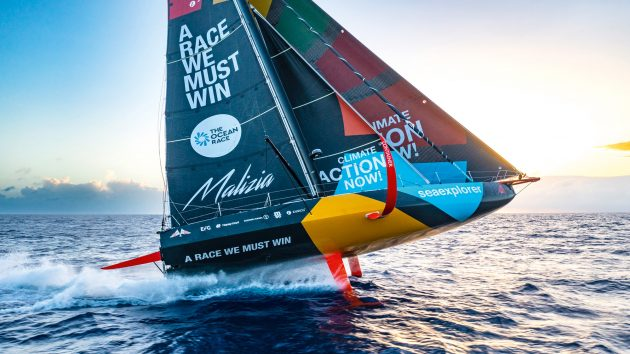
\includegraphics[width=0.42\textwidth]{resources/img/chapter1/boat.png}
    \caption{The IMOCA 60 \emph{Malizia Seaexplorer}, one of the world's fastest monohulls.}
    \label{fig:imoca}
    \vspace{-17pt}
\end{wrapfigure}
The application of Deep Reinforcement Learning (DRL) in autonomous navigation and control is becoming increasingly ubiquitous. In the context of autonomous sailing, DRL addresses a high dimensional optimal control problem characterized by nonlinear dynamics and significant environmental uncertainties. The ability of a DRL agent to learn this control problem directly correlates with performance improvements in elite competitive environments, such as the solo round the world Vendée Globe\footnote{The Vendée Globe is a non stop, round the world yacht race widely regarded as one of the most demanding sailing competitions.}. Racing environments often employ a specialized class of vessel known as a \emph{sailboat}. Compared to traditional motorized vessels sailboats operate without an engine and they rely entirely on wind as their primary power source. Nevertheless, modern racing sailboats are equipped with sophisticated autopilot systems that are essential for both sailor safety and competitive performance. Figure~\ref{fig:imoca} illustrates the IMOCA 60 class sailboat, representing the pinnacle of technological innovation and navigational complexity in offshore racing.

\justify These sailboats transform navigation into a complex strategic problem in which every decision must reconcile nonlinear aerodynamic and hydrodynamic interactions with continuously evolving environmental conditions. One can naturally formulated this navigation task as a \emph{Markov Decision Process (MDP)}. A key limitation of current systems is that they typically rely on closed loop control\footnote{Closed-loop control continuously adjusts actions based on feedback from the current system state, e.g., via PID controllers.}  to maintain a fixed heading or apparent wind angle, without explicitly optimizing trajectory efficiency or speed. Under volatile conditions, human sailors often need to intervene manually to remain competitive. Maximizing the boat's velocity toward an upwind target (the Course Made Good (CMG) requires continuous adaptation to stochastic environmental variables such as fluctuating wind vectors and changing sea states.




\justify Reinforcement learning (RL) offers a natural framework for addressing the challenges of sequential decision making under uncertainty. In the traditional machine learning (ML) paradigm, supervised learning relies on labeled datasets to map inputs to known outputs, while unsupervised learning seeks to identify hidden patterns within unlabeled data. Deep Reinforcement Learning (DRL) in contrast, enables an agent to discover optimal behavior through trial and error. It operates as a sequential decision making framework in which the agent learns to select actions via continuous interaction with an environment, guided by feedback signals in the form of \emph{rewards}. The agent's objective is to maximize cumulative reward over time. The “deep” component refers to the use of deep neural networks to approximate policies or value functions allowing learning in complex, high dimensional environments. Traditional ML and classical control methods are often unsuitable for the “strategy under uncertainty” required in sailing. Supervised learning fails because there is rarely a comprehensive labeled dataset covering every combination of wave height, wind gusts, and sea state. Similarly, rule based controllers or classical PID schemes require explicit physical models, which struggle to capture the nonlinear interactions between the sails and dynamic ocean environment.


\subsection{Principles of Sailboat Dynamics}
Understanding the physical foundations of sailboat behavior is critical for designing effective RL agents. Sailboats are generally categorized into two types based on the number of buoyant hulls. \textbf{Monohulls} utilize a single hull with a heavy ballast to provide stability, while \textbf{Multihulls} achieve stability through a wider beam and multiple hulls. Regardless of body type, the interaction between the vessel and its environment is governed by several core structural components. Figure~\ref{fig:boats} illustrates these key architectural elements in real-world sailboats. \textbf{The Keel:} A fixed structure extending beneath the hull (Figure~\ref{fig:boats} A,B), the keel serves a dual function: generating a righting moment to resist heeling and producing hydrodynamic lift to minimize leeway (sideways drift). \textbf{The Rudder:} The primary steering mechanism (Figure~\ref{fig:boats} D), the rudder creates a turning moment by deflecting water flow, allowing the sailor (or agent) to adjust the boat’s relative heading ($\beta$) and maintain the desired trajectory.


\begin{figure}[H]
    \centering
    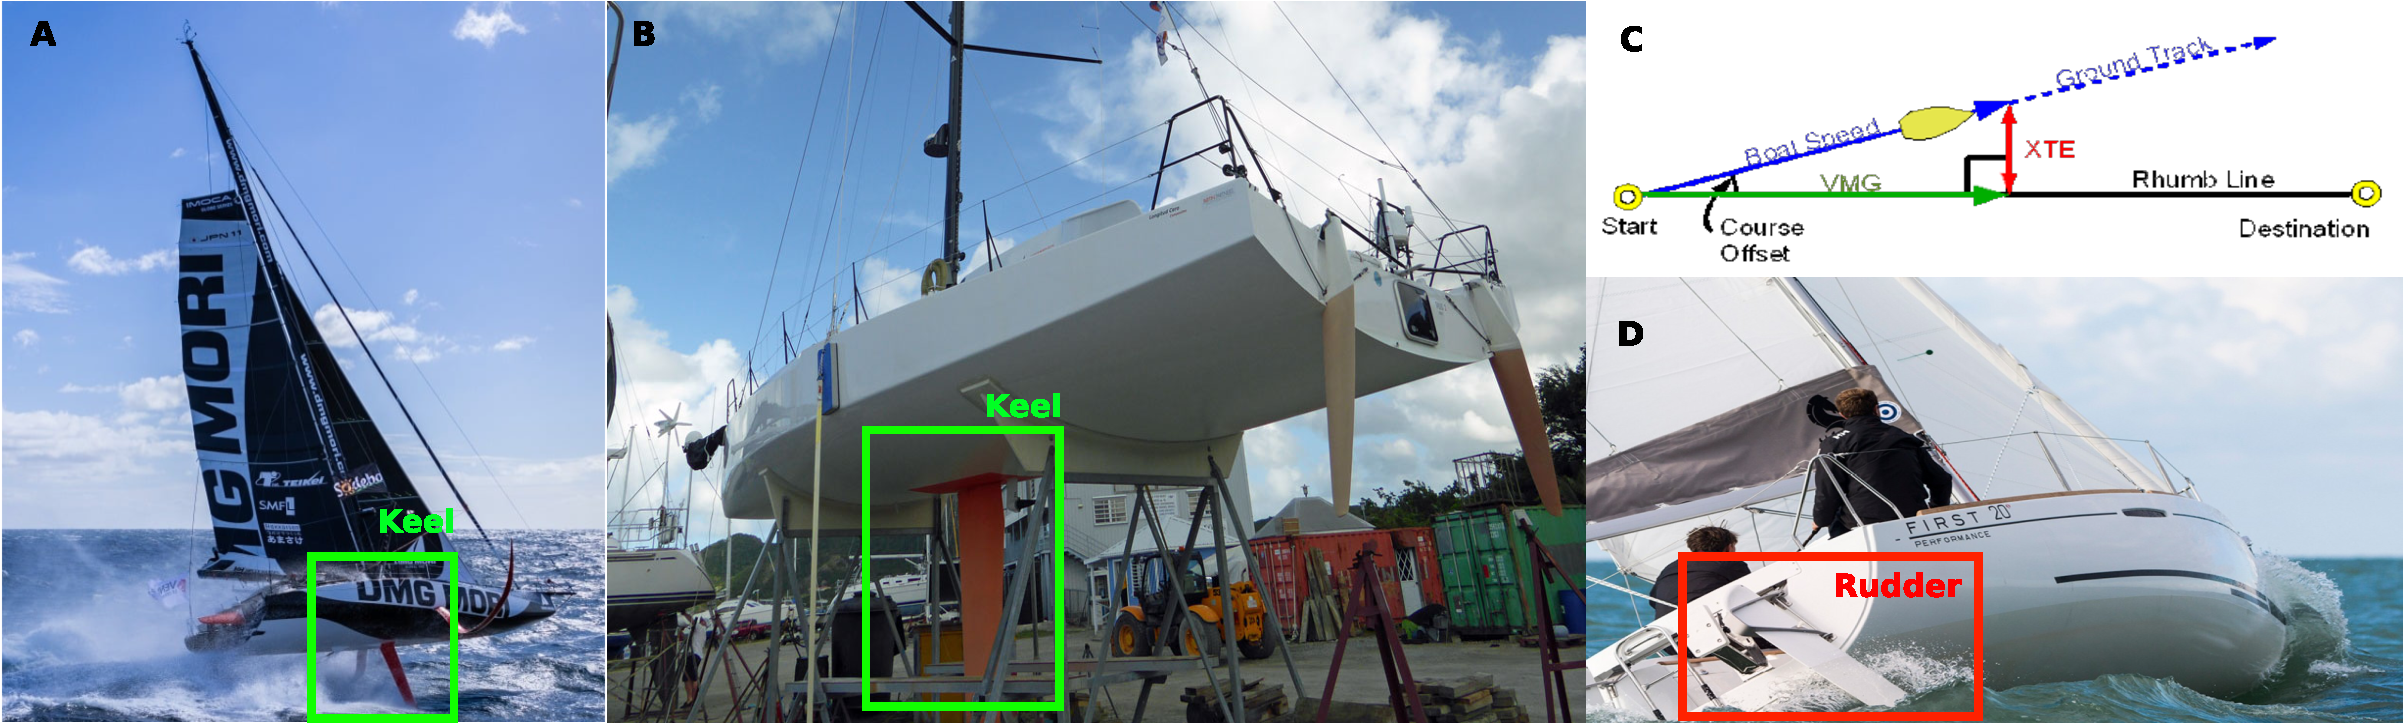
\includegraphics[width=1\linewidth]{resources/img/chapter1/boats_keel.pdf}
    \caption{Sailing dynamics and components of a sailboat. (A \& B) showing the keel (green) for lateral stability. 
    (C) Vector diagram of CMG, course offset, and cross-track error (XTE). 
    (D) Stern close-up showing the rudder (red) for steering.}
    \label{fig:boats}
\end{figure}

\justify The motion of a sailboat is governed by a dynamic equilibrium of Newtonian forces and fluid structure interactions. Propulsion is primarily generated through the \textbf{Coandă Effect}, in which airflow sticks to the curvature of the sail and is redirected backward. According to Newton’s Third Law, this deflection produces an equal and opposite reaction force, resulting in a total aerodynamic force. A component of this force provides the forward thrust ($F_{\text{thrust}}$) necessary to accelerate the vessel to a given velocity ($V_{\text{boat}}$). The net acceleration of the boat can be expressed:
\[
F_{\text{net}} = F_{\text{thrust}} - F_{\text{drag}},
\]
\justify where $F_{\text{drag}}$ includes both aerodynamic resistance and hydrodynamic friction. Maintaining directional efficiency requires a precise control: the keel converts lateral wind pressure into forward motion, while the rudder enables steering at the cost of minor “steering drag.” Mastery of this balance between air and water forces is the ultimate challenge that the RL agent must learn to optimize performance. 

\justify Beyond raw acceleration, the efficiency is measured by its progress toward a target destination. This is quantified by the Course Made Good (CMG), which represents the effective velocity projected onto the intended path. Given a course offset angle $\beta$—the angle between the boat’s heading and the target line CMG is defined as:  
\begin{equation}
    \text{CMG} = V_{\text{boat}} \cdot \cos(\beta)
\end{equation}


\justify Simultaneously, the agent must minimize the Cross-Track Error (XTE), the perpendicular distance from the current position to the target trajectory. If $D$ denotes the distance traveled from the starting point, lateral deviation is expressed as:

\begin{equation}
    \text{XTE} = D \cdot \sin(\beta)
\end{equation}

By optimizing $F_{\text{net}}$ to maintain speed while minimizing XTE, the sailors (agent) maximizes CMG along the most direct trajectory, achieving both efficient propulsion and precise navigation.

%%%%%%%%%%%%%%%%%%%%%%%%%%%%%%%%%%%%%%%%%%%%%%%%%%%%%%%%%%%%%%%%

\subsection{Problem Definition and Navigation Challenge} 
The primary objective of this project is to explore how DRL can extend traditional autopilot capabilities beyond simple set point maintenance, evolving them into intelligent systems capable of strategic navigation under uncertainty.

\subsubsection{Simulation Environment: \emph{BoatSimulator}} 
This study employs a high fidelity Python-based simulation environment called \emph{BoatSimulator}\footnote{Developed at Nautia}, built using the OpenAI Gymnasium framework to model boat dynamics in open sea conditions. For RL compatibility, the simulator is packaged within \emph{boatsgym}, a wrapper compliant with the Gymnasium API. The graphical user interface (GUI) and 3D visualization of the BoatSimulator are presented in Figure \ref{fig:simg}. 

\begin{figure}[H]
    \centering
    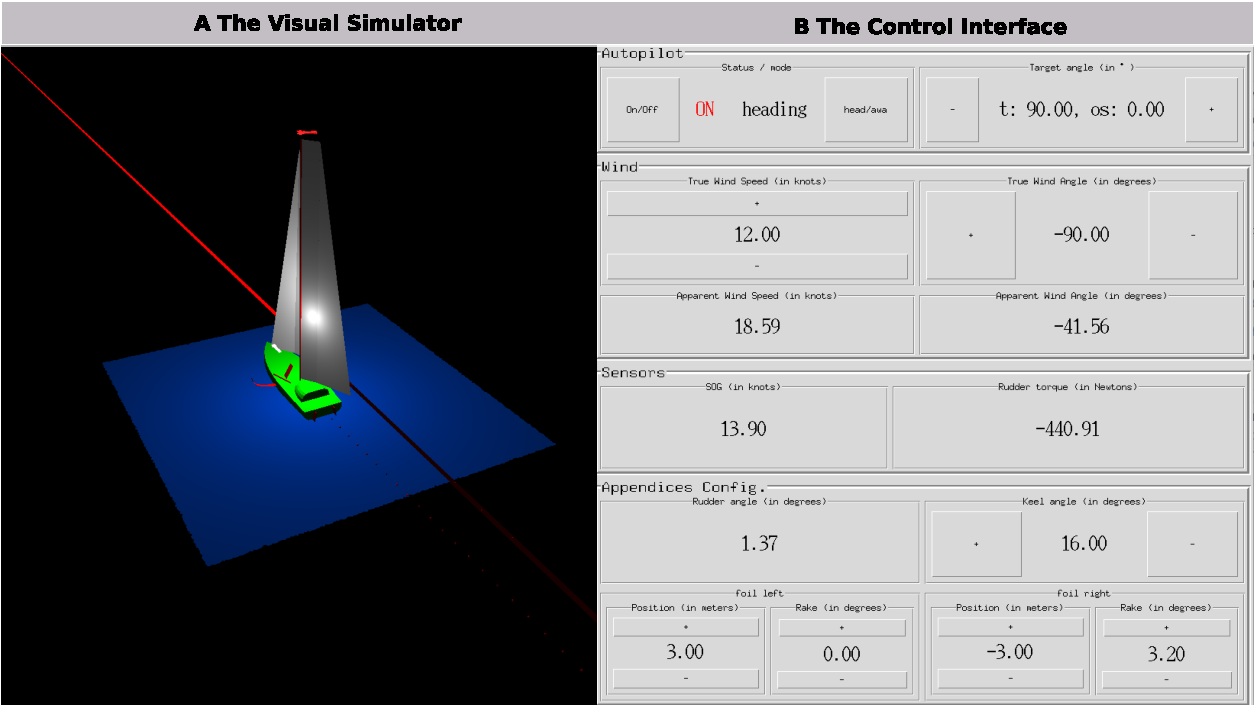
\includegraphics[width=1\linewidth]{resources/img/chapter1/simulator.pdf}
    \caption{The \emph{BoatSimulator} interface, featuring the system control dashboard (left) and 3D environmental viewport (right).}
    \label{fig:simg}
\end{figure}

At the core of the navigation logic in the BoatSimulator is a classical Proportional-Integral-Derivative (PID) control loop which serves as the baseline for this study.

\subsubsection{Baseline PID Performance and Navigation Limitations}

Figure \ref{fig:traje} illustrates a scenario in which the BoatSimulator's PID controller attempts to maintain a target heading of $90^\circ$ under a 12 kt wind. While the controller successfully stabilizes the boat's orientation, a persistent lateral deviation (called leeway) remains. This Cross-Track Error (XTE), visualized as the vertical red lines between the observed path and the target trajectory, arises because the PID controller only regulates angular heading and lacks awareness of the boat’s global position and effective forward progress. As a result although the heading is maintained, the sailboat drifts sideways relative to the intended trajectory, limiting its CMG. 

\begin{figure}[H] 
    \centering 
    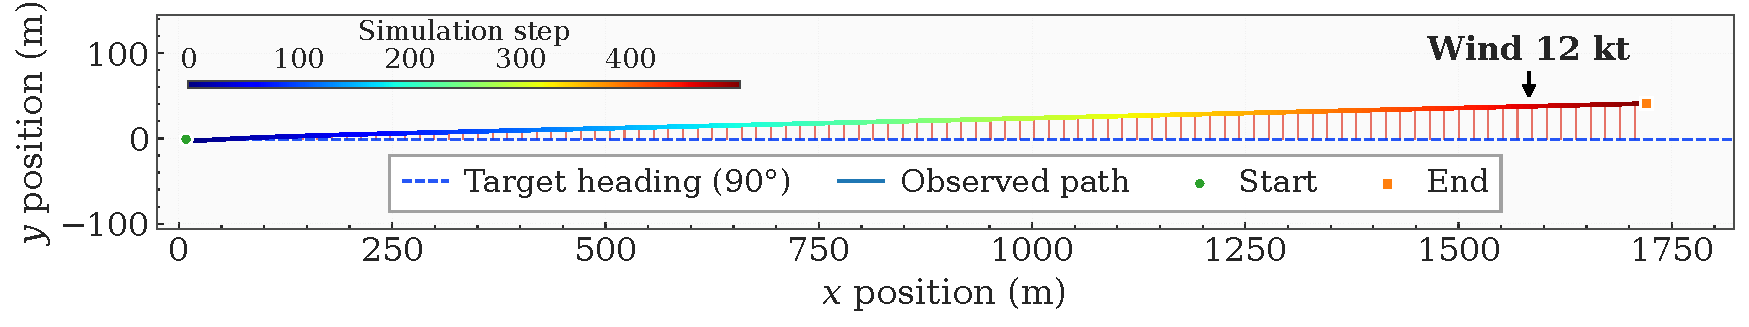
\includegraphics[width=1\linewidth]{resources/img/chapter1/trajectory_xte_pub.pdf} 
    \caption{Trajectory toward $90^\circ$ under 12 kt wind. The blue dashed line represents the target trajectory, while the vertical red lines indicate the accumulation of XTE despite stable heading control.} 
    \label{fig:traje}
\end{figure}

The performance implications of the PID controller’s limitations are further illustrated in Figure \ref{fig:pid-performance}. The CMG reward representing the component of the boat’s velocity aligned with the target trajectory initially spikes as the vessel accelerates but ultimately stabilizes at a sub-optimal mean of $13.89\,\text{m/s}$. Corresponding control plots indicate that the heading error converges to a small non zero value, while the rudder angle stabilizes near $80^\circ$ to counteract wind forces. Despite these stabilizations, the system fails to maximize forward velocity toward the goal.

\begin{figure}[H] 
    \centering 
    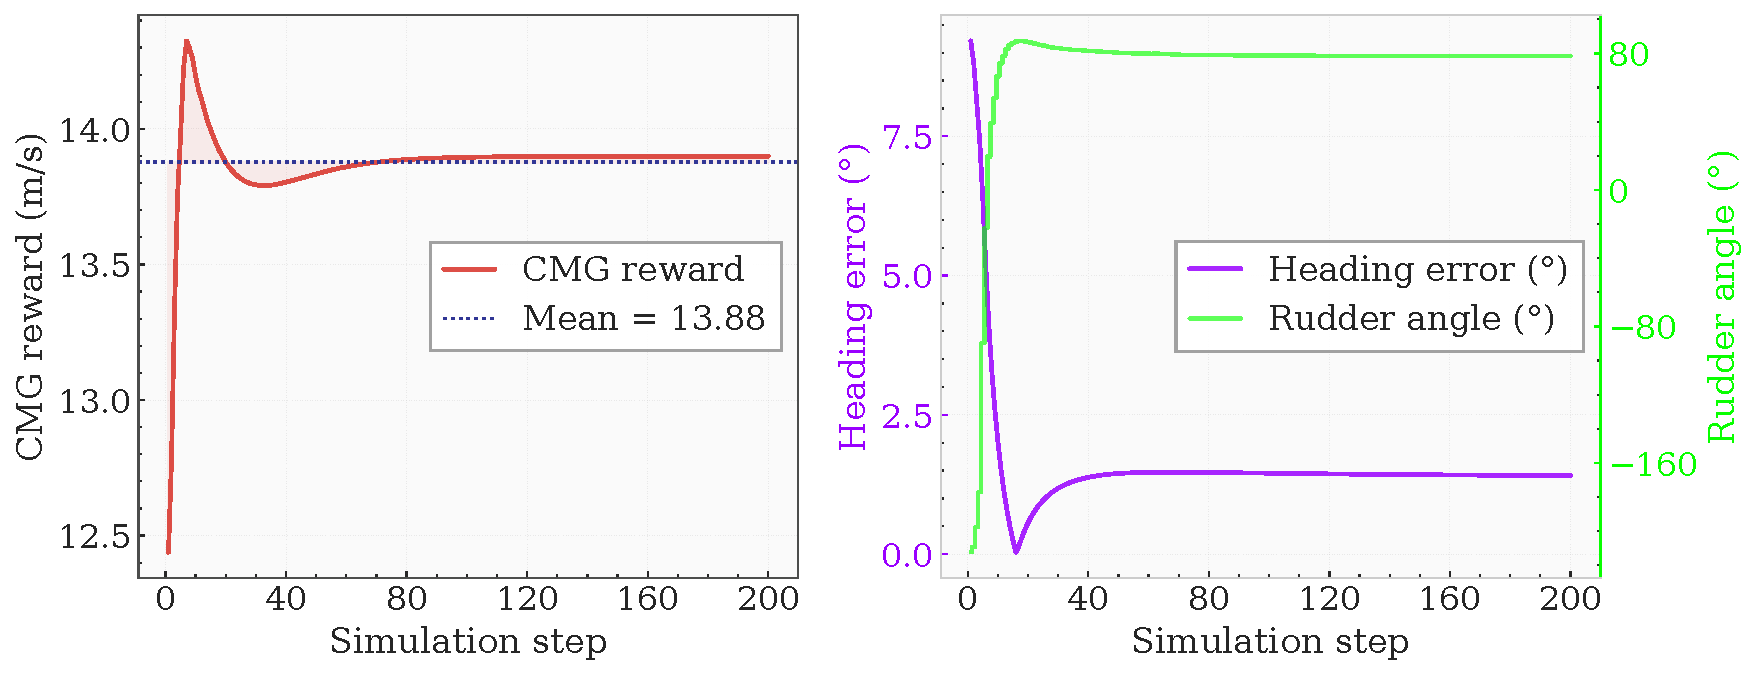
\includegraphics[width=1\linewidth]{resources/img/chapter1/cmg_control_first200_pub.pdf} 
    \caption{Baseline PID performance metrics. \textbf{Left:} CMG reward over time. \textbf{Right:} Heading error and rudder angle stabilization under constant environmental forcing.} 
    \label{fig:pid-performance} 
\end{figure}

Maintaining a constant heading alone is insufficient for maximizing forward progress (CMG). To address this limitation of classical closed-loop controllers, a DRL agent must learn to combine precise heading control with a strategy that proactively maximizes CMG, adapting continuously to stochastic environmental forces and moving beyond the constraints of simple set point regulation.
%newpage
\section{Proximal Policy Optimization (PPO) Algorithm}


Reinforcement Learning (RL) spans a wide range of algorithms designed to enable an agent to learn optimal behavior through interactions with its environment. This interaction is formally modeled as a Markov Decision Process (MDP) represented by the tuple $(\mathcal{S}, \mathcal{A}, P, R, \gamma)$. Here, $\mathcal{S}$ denotes the set of all possible states of the environment (such as the sailboat's position, CMG, and wind angle), while $\mathcal{A}$ represents the set of all possible actions (such as turn left, turn right or maintain heading rudder via rudder corrections). The transition dynamics are encoded by the probability function $P(s'|s,a)$, which gives the likelihood of reaching state $s'$ after taking action $a$ in state $s$. The scalar reward function $R(s,a)$ provides feedback on the quality of actions (such as CMG). Finally, the discount factor $\gamma \in [0,1]$ balances the importance of immediate versus future rewards guiding the agent toward long term optimal behavior.

\begin{figure}[H]
    \centering
    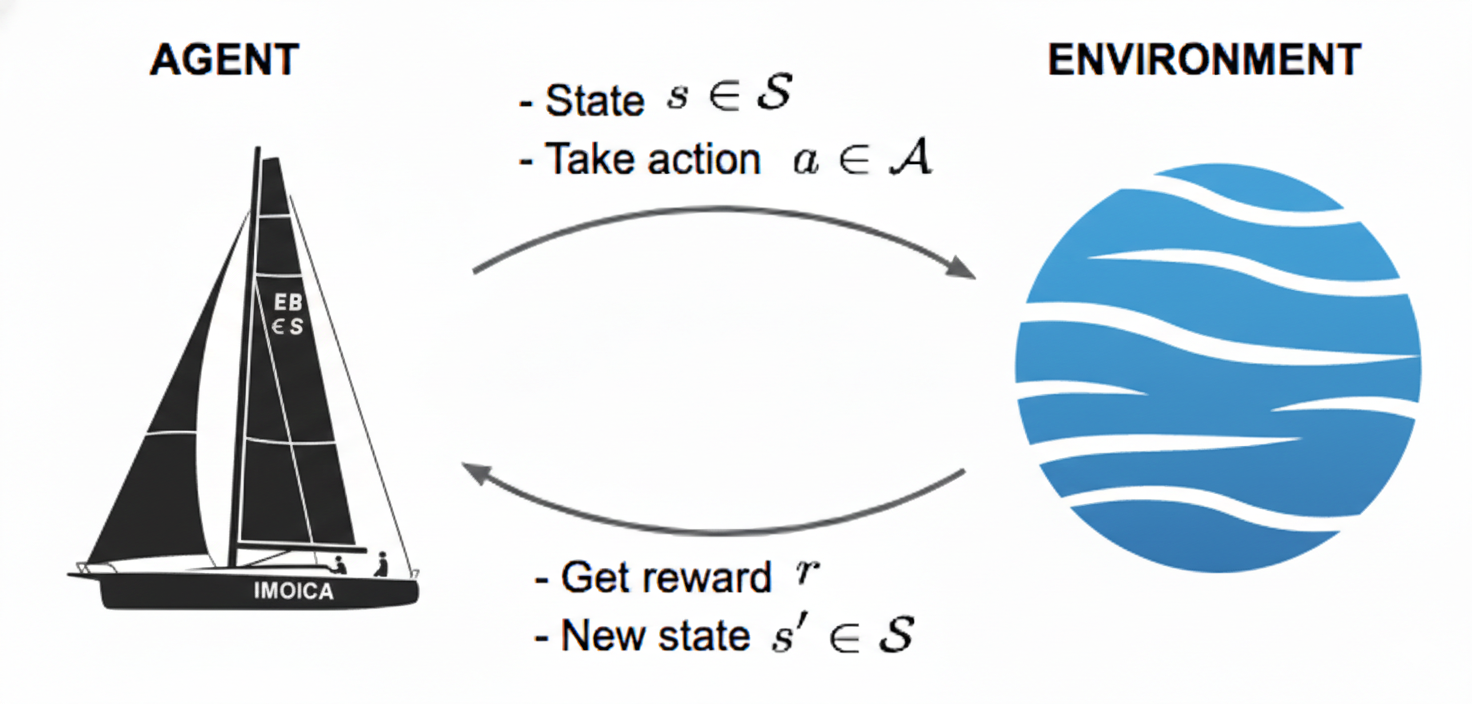
\includegraphics[width=0.6\linewidth]{resources/img/Gemini_Generated_Image_rhs7gfrhs7gfrhs7.png}
    \caption{ Markov Decision Process (MDP) of Reinforcement Learning}
    \label{fig:placeholder}
\end{figure}

\justify A \textbf{policy}, denoted as $\pi(a|s)$, is a mapping from states to a probability distribution over actions. It encodes the agent's behavior: given a state $s$, the policy defines the likelihood of taking each possible action $a$. The objective of RL is to learn an optimal policy $\pi^*$ that maximizes the expected cumulative reward over time:

\begin{equation}
J(\pi) = \mathbb{E}_{\tau \sim \pi} \Bigg[ \sum_{t=0}^{T} \gamma^t r(s_t, a_t) \Bigg],
\end{equation}

where $\tau = (s_0, a_0, s_1, a_1, \dots)$ denotes a trajectory generated by following policy $\pi$.

\justify To optimize this objective, \textbf{Policy Gradient methods} directly parameterize the policy and update it to increase the probability of actions that yield a high advantage (performing better than average). This approach is naturally suited for continuous action spaces and stochastic policies.



\subsection{From Policy Gradients to PPO}

\justify Vanilla policy gradient methods can be unstable due to large parameter updates. Trust region methods such as TRPO stabilize learning by constraining policy updates within a KL-divergence-based region, but they require complex second-order optimization. PPO simplifies this approach by introducing a \emph{clipped surrogate objective} that constrains the update magnitude while remaining compatible with first-order optimization.  

\justify In PPO, a probability ratio is defined between the new policy $\pi_\theta$ and the old policy $\pi_{\theta_\text{old}}$:

\begin{equation}
r_t(\theta) = \frac{\pi_\theta(a_t|s_t)}{\pi_{\theta_\text{old}}(a_t|s_t)}.
\end{equation}

The clipped objective is then:

\begin{equation}
L^\text{CLIP}(\theta) = \mathbb{E}_t \Big[ \min \big( r_t(\theta) A_t, \ \text{clip}(r_t(\theta), 1-\epsilon, 1+\epsilon) A_t \big) \Big],
\end{equation}

where $\epsilon$ (e.g., 0.2) sets the clipping threshold, and \(A_t\) is estimated by GAE. This objective ensures that updates do not move the policy too far in a single step, providing a “pessimistic” lower bound: policy changes that would improve the objective beyond the threshold are ignored, while detrimental changes are penalized.



\subsection{Hyperparameter Selection and Adaptation for Sailboat Navigation}
\label{sec:hyp}
\justify PPO performance is sensitive to several hyperparameters. The rollout horizon $T$ defines the number of steps over which the agent collects experience before updating the policy. While canonical papers use $T=2048$ for complex robotics tasks, we selected $T=128$ steps (corresponding to 60 seconds) to ensure frequent updates that can respond effectively to rapidly changing wind and wave conditions. The discount factor $\gamma$ balances immediate versus delayed rewards; with $\gamma=0.995$, the agent accounts for the delayed effect of rudder inputs on CMG, preventing shortsighted behavior. To reduce variance in noisy environments, the Generalized Advantage Estimator (GAE) parameter $\lambda$ was set to 0.92, slightly lower than the typical 0.95 in robotics benchmarks, which helps smooth high-frequency fluctuations from waves while capturing the underlying navigation strategy. The clipping parameter $\epsilon=0.2$ ensures that policy updates remain within a safe "trust region," preventing large, destabilizing changes when sudden wind gusts occur. A linearly decayed learning rate from $10^{-3}$ to $10^{-5}$ allows the agent to first learn basic sailing dynamics before fine-tuning maneuvers for optimal CMG. Exploration is encouraged through an entropy bonus $c_2 = 0.01$, preventing the agent from settling into sub-optimal, overly conservative rudder strategies. Finally, the neural network architecture employs a lightweight $64 \times 64$ MLP, providing sufficient capacity for learning the mapping from environmental states to actions while remaining compatible with real-time control at 2 Hz. Overall, these adaptations reflect a careful balance between literature-recommended defaults and the unique dynamics and stochasticity of autonomous sailboat navigation.


\section{State of the Art in Autonomous Sailing Agents}

\subsection{Implementation Framework and Training Protocol}
The state of the art RL agent was developed using the \texttt{PyTorch} deep learning library and the \texttt{Stable Baselines3} (SB3) framework. Each training experiment spanned 250,000 timesteps, and a multi-seed evaluation strategy ($N_{\text{seeds}}=2$) was employed to ensure statistical robustness. Raw environmental observations, originally provided as hierarchical data structures, were processed through a \texttt{FlattenObservation} wrapper to produce a 1D feature vector. A \texttt{VecNormalize} wrapper was used to standardize observations and rewards to zero mean and unit variance. Additionally, a \texttt{CheckpointCallback} was invoked every 5,000 steps to archive model parameters and track agent performance throughout training.

\justify To address the substantial computational and energy demands associated with long horizon RL training, we developed \textbf{\texttt{NonDaemonicSubprocVecEnv}} architecture. This framework enables synchronous parallel data collection across multiple environments, significantly reducing wall clock training time. Unlike standard vectorized environments, this custom implementation uses non-daemonic child processes\footnote{A non-daemonic child process operates independently of the main program's exit status and is permitted to spawn its own sub-processes.}. This design not only accelerates policy convergence but also aligns with \emph{Green carbon} objectives by maximizing hardware utilization and improving the overall energy efficiency of the computational pipeline.


\begin{table}[h]
\centering
\begin{tabular}{ll}
\hline
\textbf{Hyperparameter} & \textbf{Value} \\
\hline
Learning Rate & $10^{-3} \rightarrow 10^{-5}$ \\
Gamma ($\gamma$) & 0.995 \\
GAE Lambda ($\lambda$) & 0.92 \\
Batch Size & 128 \\
Entropy Coefficient & 0.01 \\
Number of Environments ($N$) & 5 \\
\hline
\end{tabular}
\caption{Hyperparameter configuration used for training the PPO agent.}
\label{tab:hyperparameters}
\end{table}
\justify Table \ref{tab:hyperparameters} summarizes the hyperparameter configuration used in this study. The learning rate was linearly decayed from $10^{-3}$ to $10^{-5}$ over the 250,000-step horizon to maintain training stability. A high discount factor ($\gamma = 0.995$) was chosen to prioritize lon term mission objectives, such as maintaining optimal CMG, over short-term high-drag maneuvers. The GAE parameter ($\lambda = 0.92$) was tuned to reduce variance in the policy gradient, while an entropy coefficient of $0.01$ was maintained to prevent premature convergence to sub optimal local minima. Training was parallelized across $N=5$ environment instances to maximize throughput and computational efficiency. This setup minimizes idle time and ensures that each subprocess has dedicated access to the simulation’s physics and graphical contexts, facilitating stable and efficient learning.

\subsection{Agent Architecture and Policy Network}
The default decision making core of the RL agent is implemented as a Multi-Layer Perceptron (MLP) within an Actor-Critic framework. Both the policy network ($\pi$) and the value function ($V$) comprise two fully connected hidden layers of 64 neurons each with a non-linear activation functions. This configuration acts as a "reactive" baseline by mapping instantaneous state observations (such as wind angle, boat speed) directly to to steering actions. While computationally efficient the standard MLP assumes that the current observation fully characterizes the environment. Foiling sailboats, however, operate in a regime where the temporal evolution of environmental variables is often as critical as their instantaneous values. The MLP treats each timestep independently, failing to capture the dynamics of wind gusts or shifting wave patterns. To remain on the foils and maximize CMG, the agent must distinguish between these transient turbulence and sustained changes in wind direction which necessitating an architecture capable of temporal reasoning.


\subsection{Temporal Feature Extraction with 1D-CNNs}


\begin{figure}[H]
    \centering
    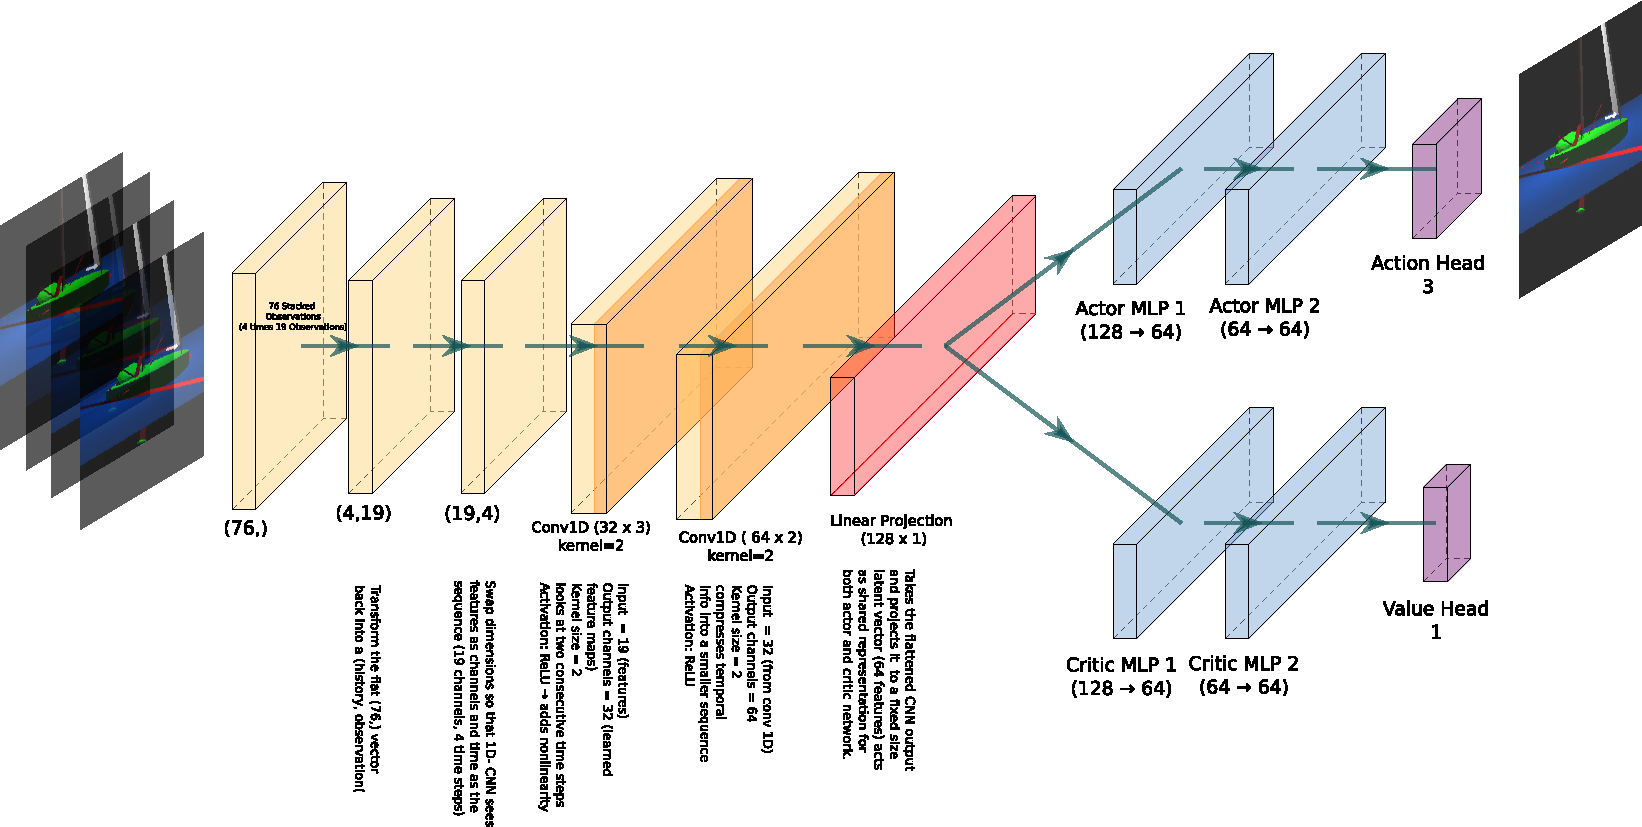
\includegraphics[width=1.0\linewidth]{resources/img/chapter3/1dcnn.pdf}
    \caption{Proposed PPO Actor-Critic network featuring a history-based 1D-CNN feature extractor. The input comprises a temporal stack of 4 consecutive observations ($\sum_{i=0}^{3} \mathbf{o}_{t-i}$). With each observation vector containing 19 physical features, the resulting 76-dimensional input is reshaped into a $(19 \text{ channels} \times 4 \text{ time steps})$ tensor. The CNN architecture employs two Conv1D layers to extract temporal patterns, which are then projected into a 64-dimensional latent representation. This embedding is shared by the Actor and Critic MLP branches to determine the optimal 3D action vector and scalar state value, respectively.}
    \label{fig:1dcnn}
\end{figure}
To address the limitations of the reactive MLP, we introduce the \textbf{HistoryCNNExtractor}, a 1D Convolutional Neural Network (1DCNN) designed to capture temporal dependencies in sailboat (see Figure \ref{fig:1dcnn}). By using a \texttt{VecFrameStack} of $n=4$ frames, the agent receives a rolling history of the environment rather than isolated snapshots. The stacked observations from the last four timesteps, $\sum_{i=1}^{4} \mathbf{o}_{t-i}$, are reshaped so that the 19 physical features are treated as channels and the four steps form the temporal dimension. This allows the convolutional kernels to slide along the time axis while observing all sensor features simultaneously at each temporal position.  

Physically, the 1D-CNN functions as a \textit{learnable differential operator}. The first convolutional layer, with a kernel size of 2, is mathematically analogous to a first-order difference operator in time:
\[
\Delta x_t = x_t - x_{t-1}.
\]
This allows the network to detect temporal trends such as the onset of wind gusts or sustained shifts in direction, providing the agent with richer information for anticipatory decision-making that improves CMG and overall sailing performance.

\begin{figure}[H]
    \centering
    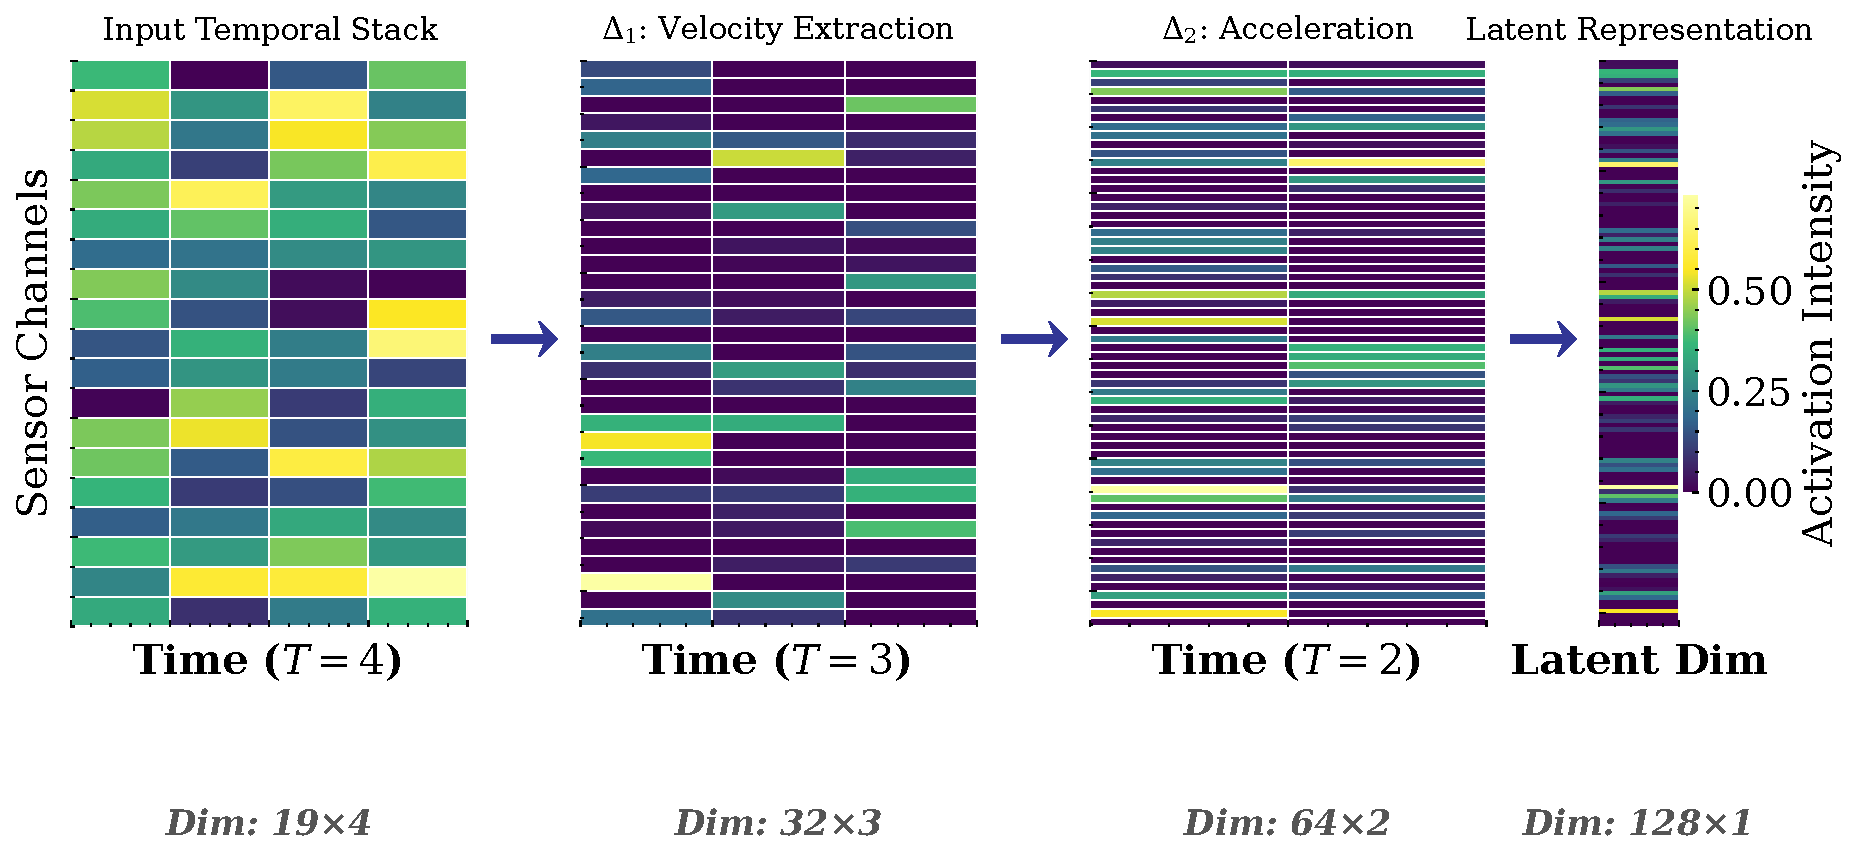
\includegraphics[width=1\linewidth]{resources/img/chapter3/dataflow_1dcnn.pdf}
    \caption{Hierarchical dataflow through the 1D-CNN feature extractor. \textbf{Panel 1:} Raw input matrix ($19 \text{ features} \times 4 \text{ steps}$). \textbf{Panel 2:} After the first convolution ($k=2$), the temporal dimension is reduced to 3; the 32 feature channels act as first-order differential operators. \textbf{Panel 3:} The second convolution reduces the temporal window to 2, processing velocity signals to extract second-order dynamics (acceleration). \textbf{Panel 4:} The latent representation, flattened to $64 \text{ channels} \times 2 \text{ steps} = 128$, provides a high-level physical abstraction for the Actor-Critic heads.}
    \label{fig:dataflow}
\end{figure}

The network autonomously extracts \emph{velocity-like} features, such as the rate of change in wind angle or boat speed. The second convolutional layer captures higher-order differences, effectively computing \emph{acceleration-like} features. With a temporal window of four frames, the network achieves sufficient depth to stabilize these derivatives against simulation noise and environmental stochasticity. The resulting high-level features are flattened into a 128-dimensional latent embedding, which is passed to the Actor-Critic heads, providing a time-aware representation of the vessel’s momentum and trajectory. As illustrated in Figure \ref{fig:dataflow}, this architecture enables the agent to go beyond reactive control, making proactive navigation decisions informed by evolving environmental trends.


\subsection{Training Protocol}
Each training episode was limited to a maximum of 512 steps, with a control frequency of $2\,\text{Hz}$ (the agent produced control decisions every 0.5 seconds). The action space is a discrete space allowing the agent to make incremental adjustments to the desired course (turn left, turn right, or maintain heading). Training was conducted under randomized environmental conditions to promote robustness and generalization. Wind speed was sampled uniformly between 10 and 18 knots, while target headings were drawn from upwind and reaching\footnote{wind comes from the side of the boat} configurations ranging from $90^\circ$ to $140^\circ$ relative to the true wind direction. Navigation precision was enforced through a narrow target definition consisting of an $8^\circ$ bearing width and a 1\,m positional tolerance, encouraging accurate trajectory tracking.

\subsubsection{Reward Design: CMG Optimization Objective}

The primary learning objective was to maximize CMG. The reward function was defined as:
\[
R = V_{\text{boat}} \cdot \cos(\theta_{\text{error})}
\]
where $V_{\text{boat}} \cdot \cos(\theta_{\text{error}})$ represents the component of velocity aligned with the target direction. The term $C_{\text{oob}}$ corresponds to a significant penalty (50 units) applied when the sailboat exits operational boundaries or loses foil stability, while $C_{\text{heading}}$ enforces a maximum deviation constraint of $45^\circ$ from the target heading.

This reward structure encourages sustained high-speed motion while maintaining directional accuracy and stable foiling behaviour.




\section{Results and Discussion}
This section presents the strategies used to obtain high performing agent and the evaluation methodology applied to compare the Baseline controller, the proactive MLP architecture and the reactive 1DCNN approach.

\subsection{Training Convergence and Optimal Checkpoint Selection}

\begin{figure}[H]
    \centering
    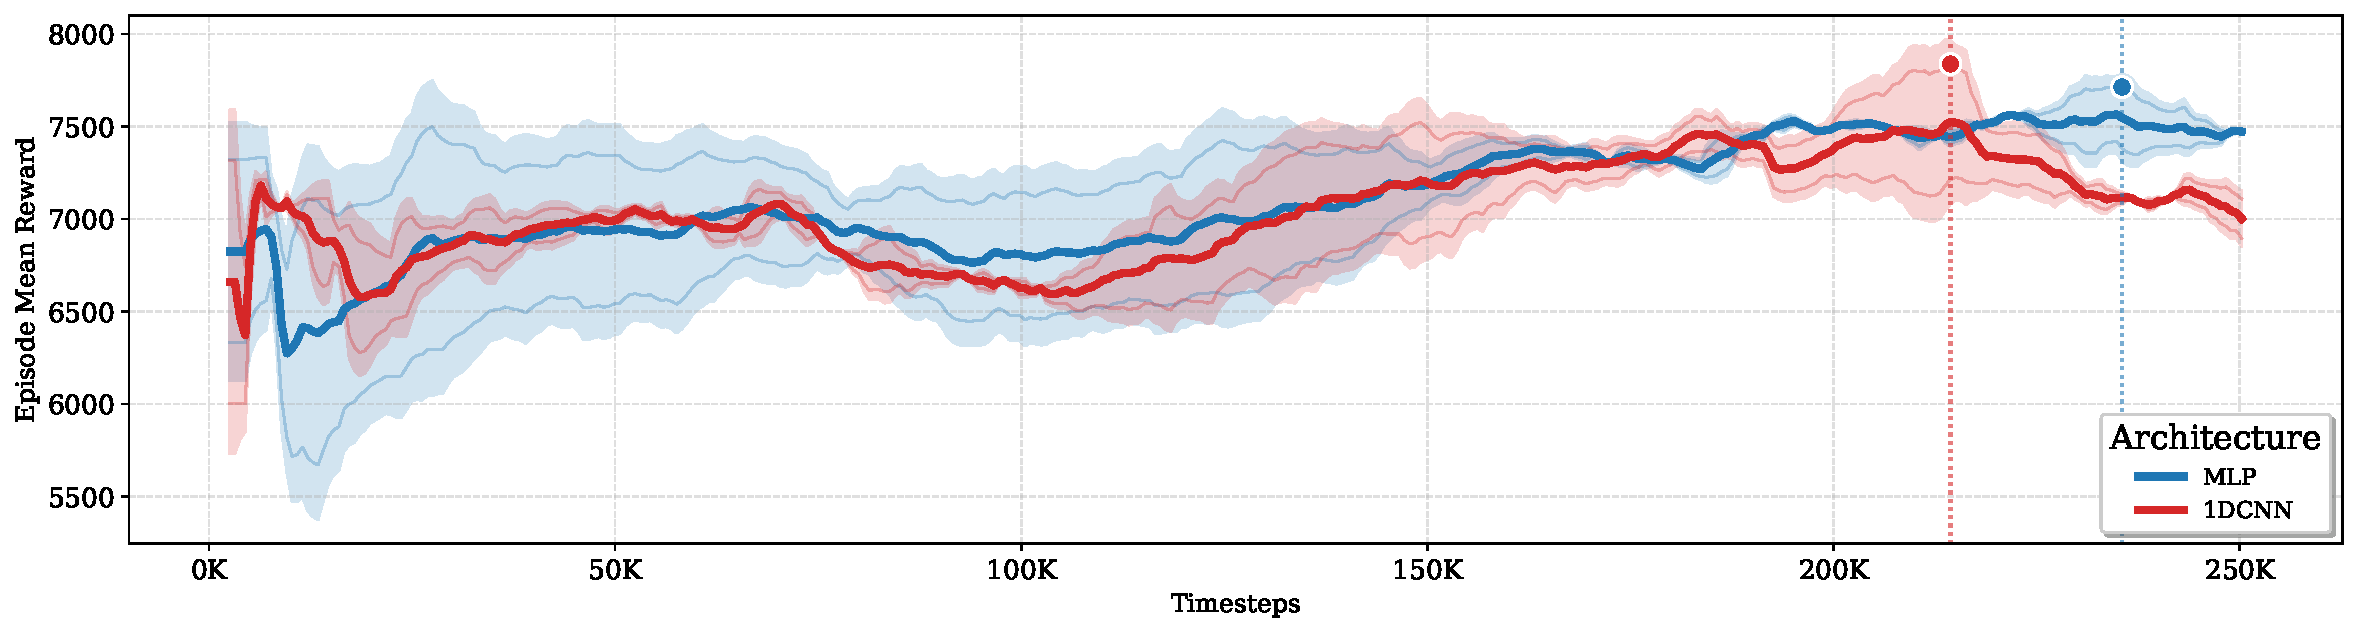
\includegraphics[width=1\linewidth]{resources/img/chapter4/ep_mean_reward.pdf}
    \caption{Training convergence and peak performance for MLP and 1DCNN architectures. Solid lines represent the exponential moving average (EMA, $\alpha=0.8$) of episode mean reward across all seeds. Shaded regions denote standard deviation ($\pm 1\sigma$), while faint trajectories correspond to individual runs. Vertical markers indicate peak performance checkpoints.}
    \label{fig:ep_mean}
\end{figure}

As illustrated in Figure~\ref{fig:ep_mean} both architectures shows a consistent upward trend in mean episodic reward, converging toward high performance plateaus exceeding $7{,}500$. The 1DCNN demonstrates improved early stage stability and reaches its peak reward faster (approximately $215$k timesteps) compared to the MLP baseline (approximately $235$k timesteps). To ensure reliable model selection two stage checkpoint selection procedure was applied: (i) identification of the maximum smoothed reward ($R_{\text{max}}$); (ii) temporal matching with the nearest saved checkpoint (stored at $5{,}000$-step intervals). The selected checkpoints were subsequently evaluated across diverse environmental conditions.

%; and (iii) downstream evaluation under standardized testing scenarios


\subsection{Evaluation Framework and Performance Metrics}
To evaluate generalization capabilities, both architectures were subjected to a deterministic evaluation suite across a combinatorial grid of 20 environmental configurations (Table \ref{tab:test_conditions}). These scenarios are categorized into three distinct regimes:

\begin{itemize}
    \item \textbf{Interpolation:} Headings of $95^{\circ}$, $115^{\circ}$, and $135^{\circ}$ assess stability within the primary training distribution.
    \item \textbf{Extrapolation:} Headings at $85^{\circ}$ and $145^{\circ}$ (positioned $5^{\circ}$ beyond the training boundaries) evaluate the graceful degradation of performance versus abrupt failure.
    \item \textbf{Stress Testing:} While wind speeds of 10, 14, and 18 knots represent trained conditions, the 20-knot scenario serves as a stress test to determine policy generalization under unobserved loads.
\end{itemize}

\begin{table}[htbp]
\centering
\caption{Evaluation Parameter Grid}
\label{tab:test_conditions}
\begin{tabular}{lc}
\hline
\textbf{Parameter} & \textbf{Testing Values} \\ \hline
Target Headings ($\theta_{target}$) & $85^{\circ}, 95^{\circ}, 115^{\circ}, 135^{\circ}, 145^{\circ}$ \\
Wind Speeds ($V_{wind}$) & $10, 14, 18, 20$ knots \\ \hline
\end{tabular}
\end{table}


\justify Feature normalization consistency was ensured by reloading the training-derived \texttt{VecNormalize} statistics. Performance was evaluated using multiple metrics: navigation precision (cross-track error and heading deviation), efficiency (CMG), and control stability (action slew rate). 

%This multidimensional evaluation framework enables detailed comparison of architectural resilience across varying environmental regimes.


\subsection{Steady-State Performance Comparison}
At the start of each navigation episode, the sailboat undergoes a transient phase before reaching stable dynamic behavior. To ensure a fair assessment of controller performance, these initial rising state were excluded from the analysis. Instead, steady state performance was evaluated using the tail segment of each episode where the control policy had converged to stable behavior. The steady state CMG was computed as

\begin{equation}
\mathrm{CMG}_{\text{steady}} = \frac{1}{T} \sum_{i = 201}^{512} \mathrm{CMG}_i,
\end{equation}

\justify where the first 200 timesteps were discarded to remove transient effects and $T = N - 200$ denotes the number of samples used for steady state averaging. Figure\ref{fig:cmg_bars} shows the $\mathrm{CMG}_{\text{steady}}$ comparison across test cases in Table \ref{tab:test_conditions}.

\begin{figure}[H]
    \centering
    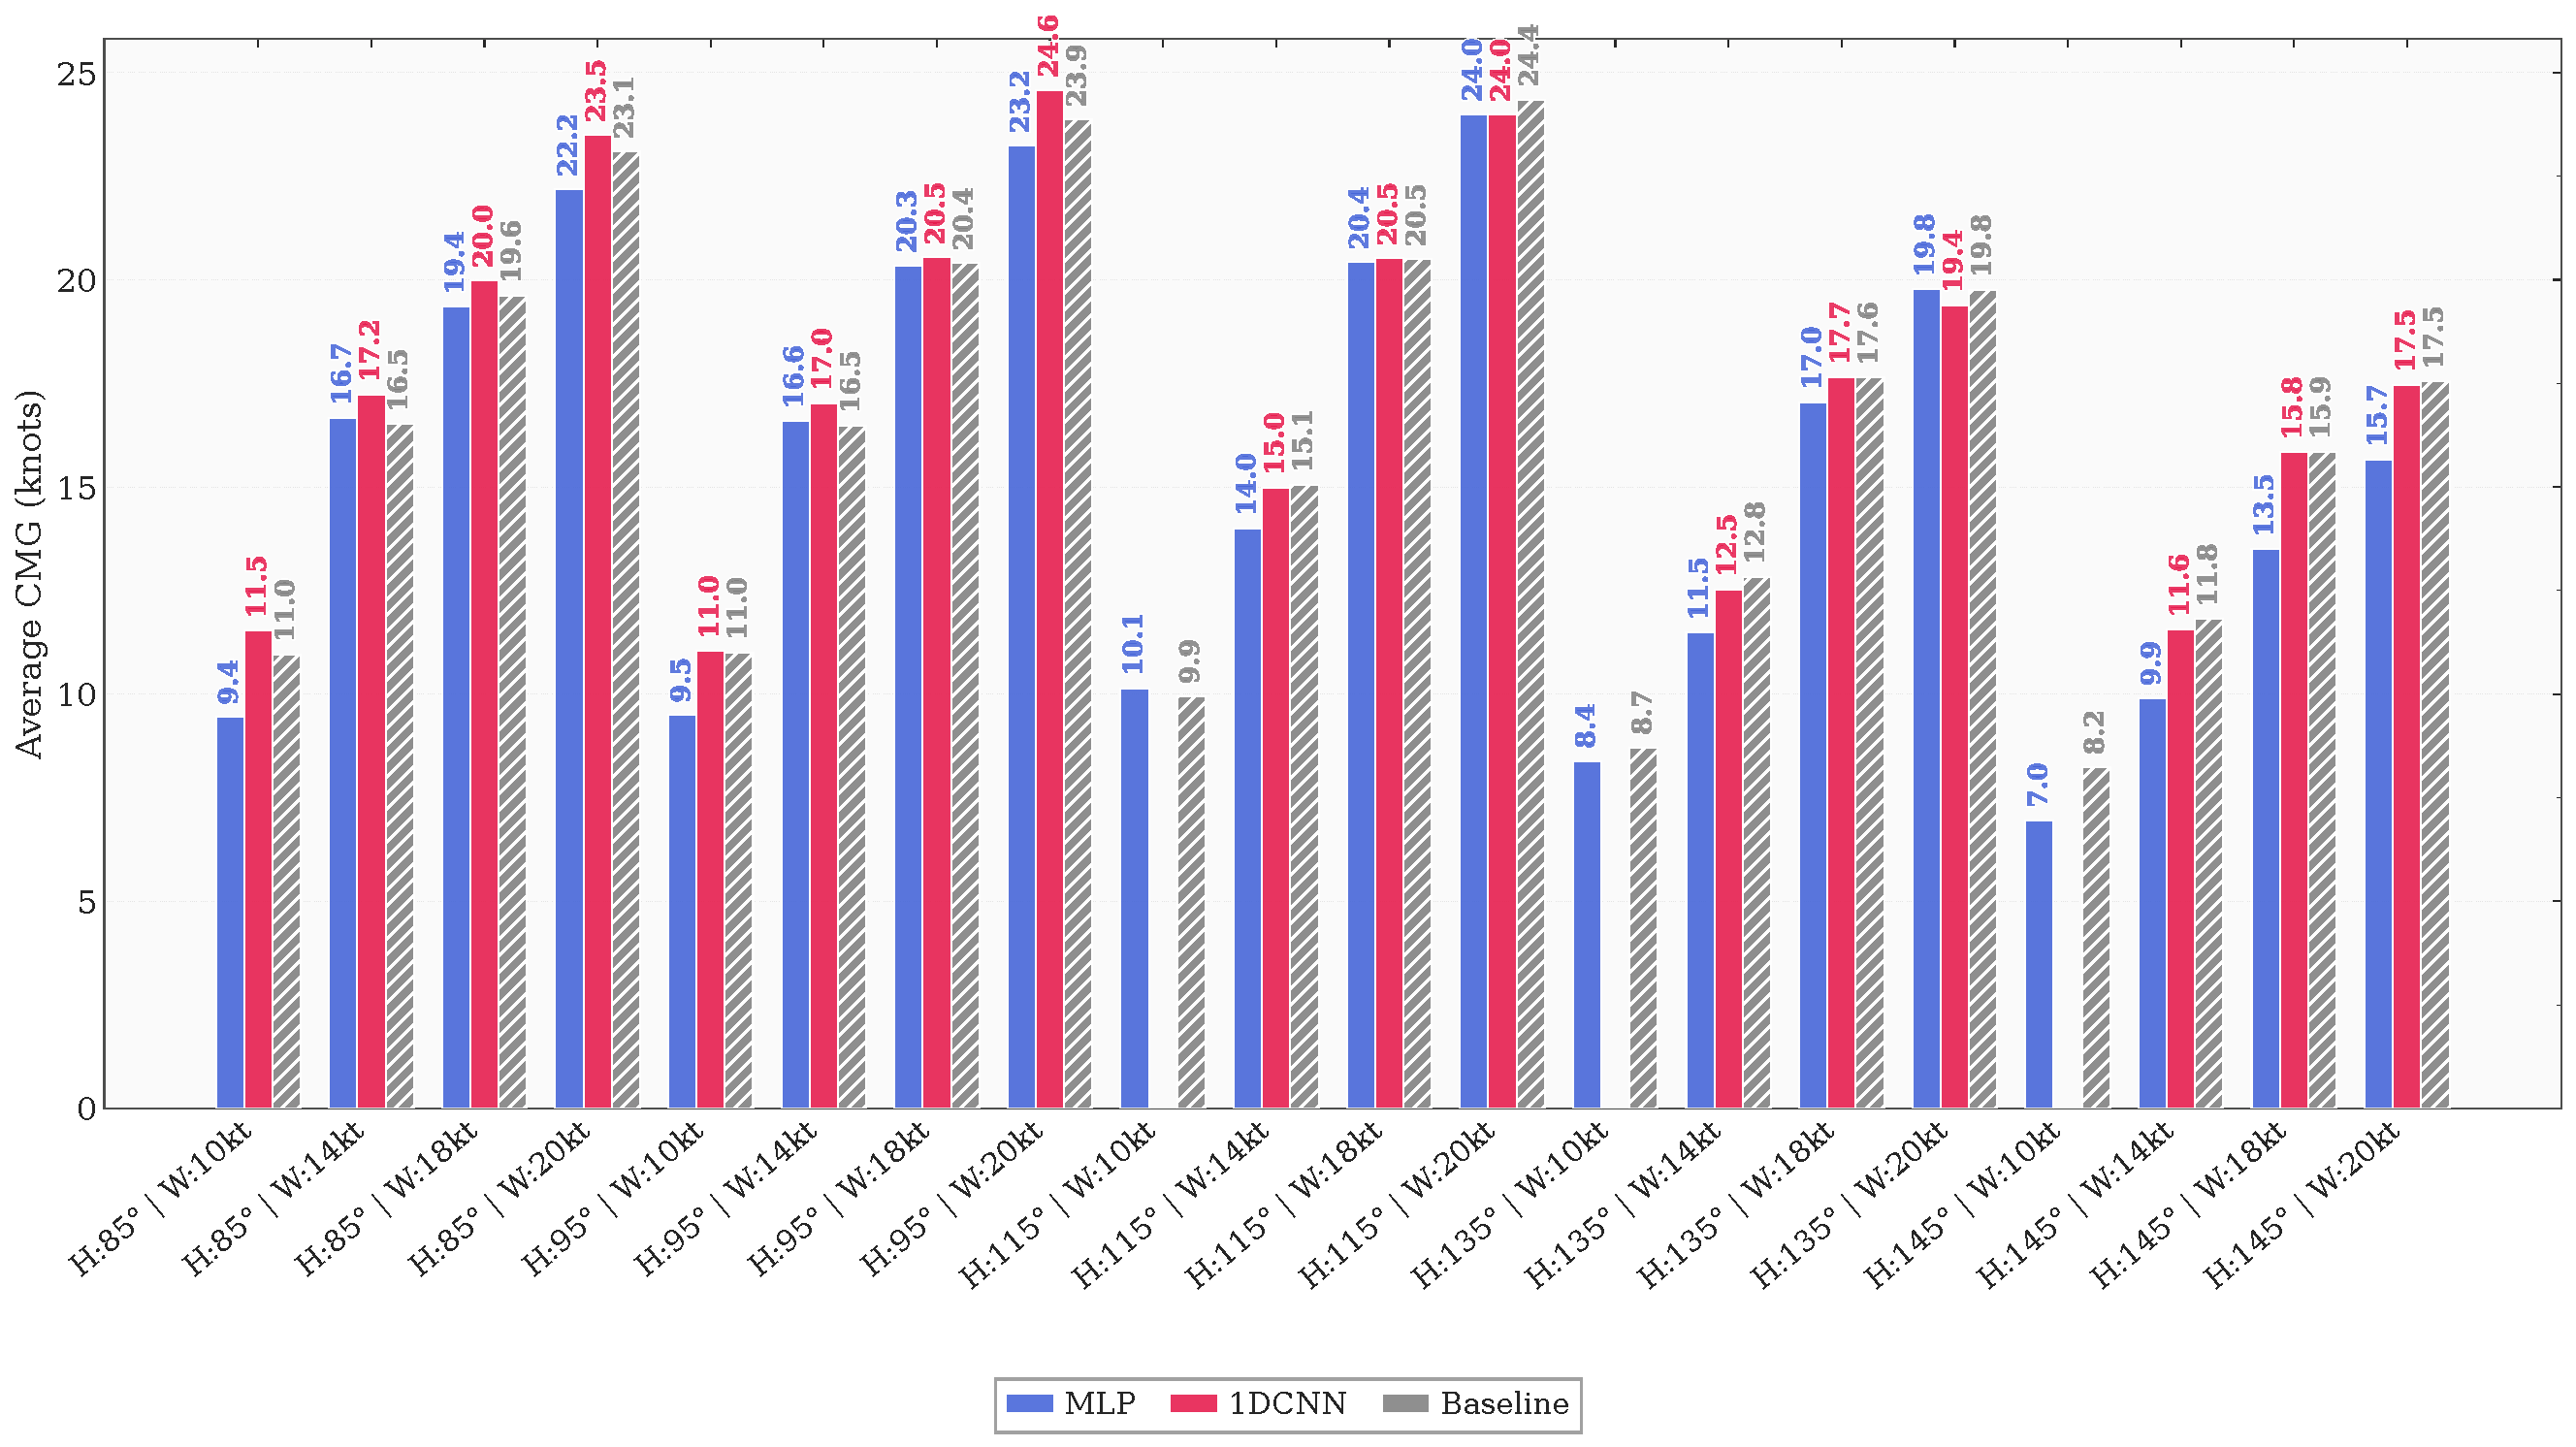
\includegraphics[width=1\linewidth]{resources/img/chapter4/per_case_cmg_comparison_pub.pdf}
    \caption{Steady-state CMG comparison across test cases. Performance differences are highlighted for out-of-distribution wind speeds ($20\,\text{kts}$) and boundary headings ($85^\circ$, $145^\circ$).}
    \label{fig:cmg_bars}
\end{figure}

 
\justify As shown in Figure~\ref{fig:cmg_bars}, both RL architectures generally outperform the baseline PID controller, which consistently achieves the lower bounds of CMG across the majority of test cases (e.g., 11.0\,kts at $H\!:\!85^\circ \mid W\!:\!14\,\text{kt}$ compared to 17.2\,kts for the 1DCNN and 16.7\,kts for the MLP). Both RL agents demonstrate strong performance and clear generalization beyond the training envelope ($H \in [90^\circ,140^\circ]$, $W \in [10,18]\,\text{kts}$). The 1DCNN emerges as the superior architecture for high-performance regimes, achieving the peak observed CMG of 24.6\,kts at $H\!:\!95^\circ \mid W\!:\!20\,\text{kt}$. Notably, the MLP exhibits significant performance degradation and policy instability under higher wind loads (18--20\,kts), whereas the 1DCNN maintains stable operation at these higher limits.
\justify However, a critical edge-case failure was identified for the 1DCNN in light-wind conditions (10\,kts) at headings $H\!:\!115^\circ$, $H\!:\!135^\circ$, and $H\!:\!145^\circ$. In these scenarios, the 1DCNN policy frequently leads to ``Out-of-Bounds'' (OOB) conditions, resulting in prematurely terminated episodes and lower average CMG values (e.g., 7.7\,kts at $H\!:\!135^\circ \mid W\!:\!10\,\text{kt}$) compared to the MLP (8.4\,kts) and baseline controller (8.7\,kts). This suggests that while the 1DCNN's temporal feature extraction excels at maximizing velocity under high loads, it may over-correct in low-energy states where the physical limits of the foils provide less damping. The polar distribution in Figure~\ref{fig:polar_plots} confirms that while the 1DCNN extends the performance frontier in the $120^\circ$ to $150^\circ$ heading range at high speeds, the MLP remains a more resilient, albeit less efficient, ``fail-safe'' option in marginal conditions.


\begin{figure}[h]
    \vspace{-3pt}
    \centering
    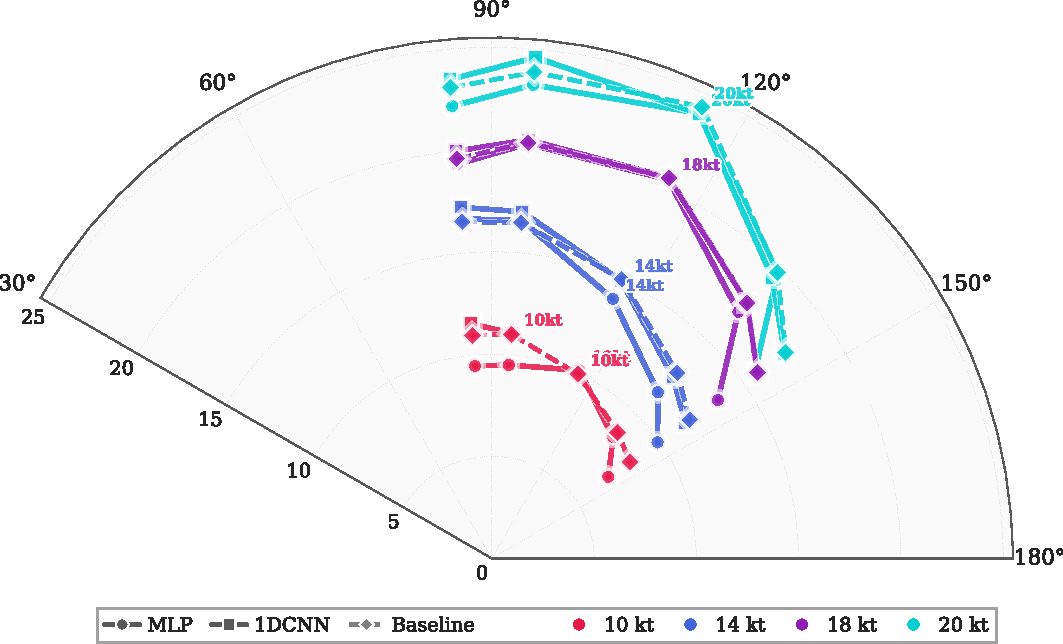
\includegraphics[width=1\linewidth]{resources/img/chapter4/polar_performance_pub.pdf}
    \caption{Polar performance distribution illustrating operational efficiency across headings. The 1DCNN maintains a broader and more consistent operational envelope.}
    \label{fig:polar_plots}
\end{figure}


\subsection{Control Dynamics and Temporal Stability}
\begin{figure}[h]
    \centering
    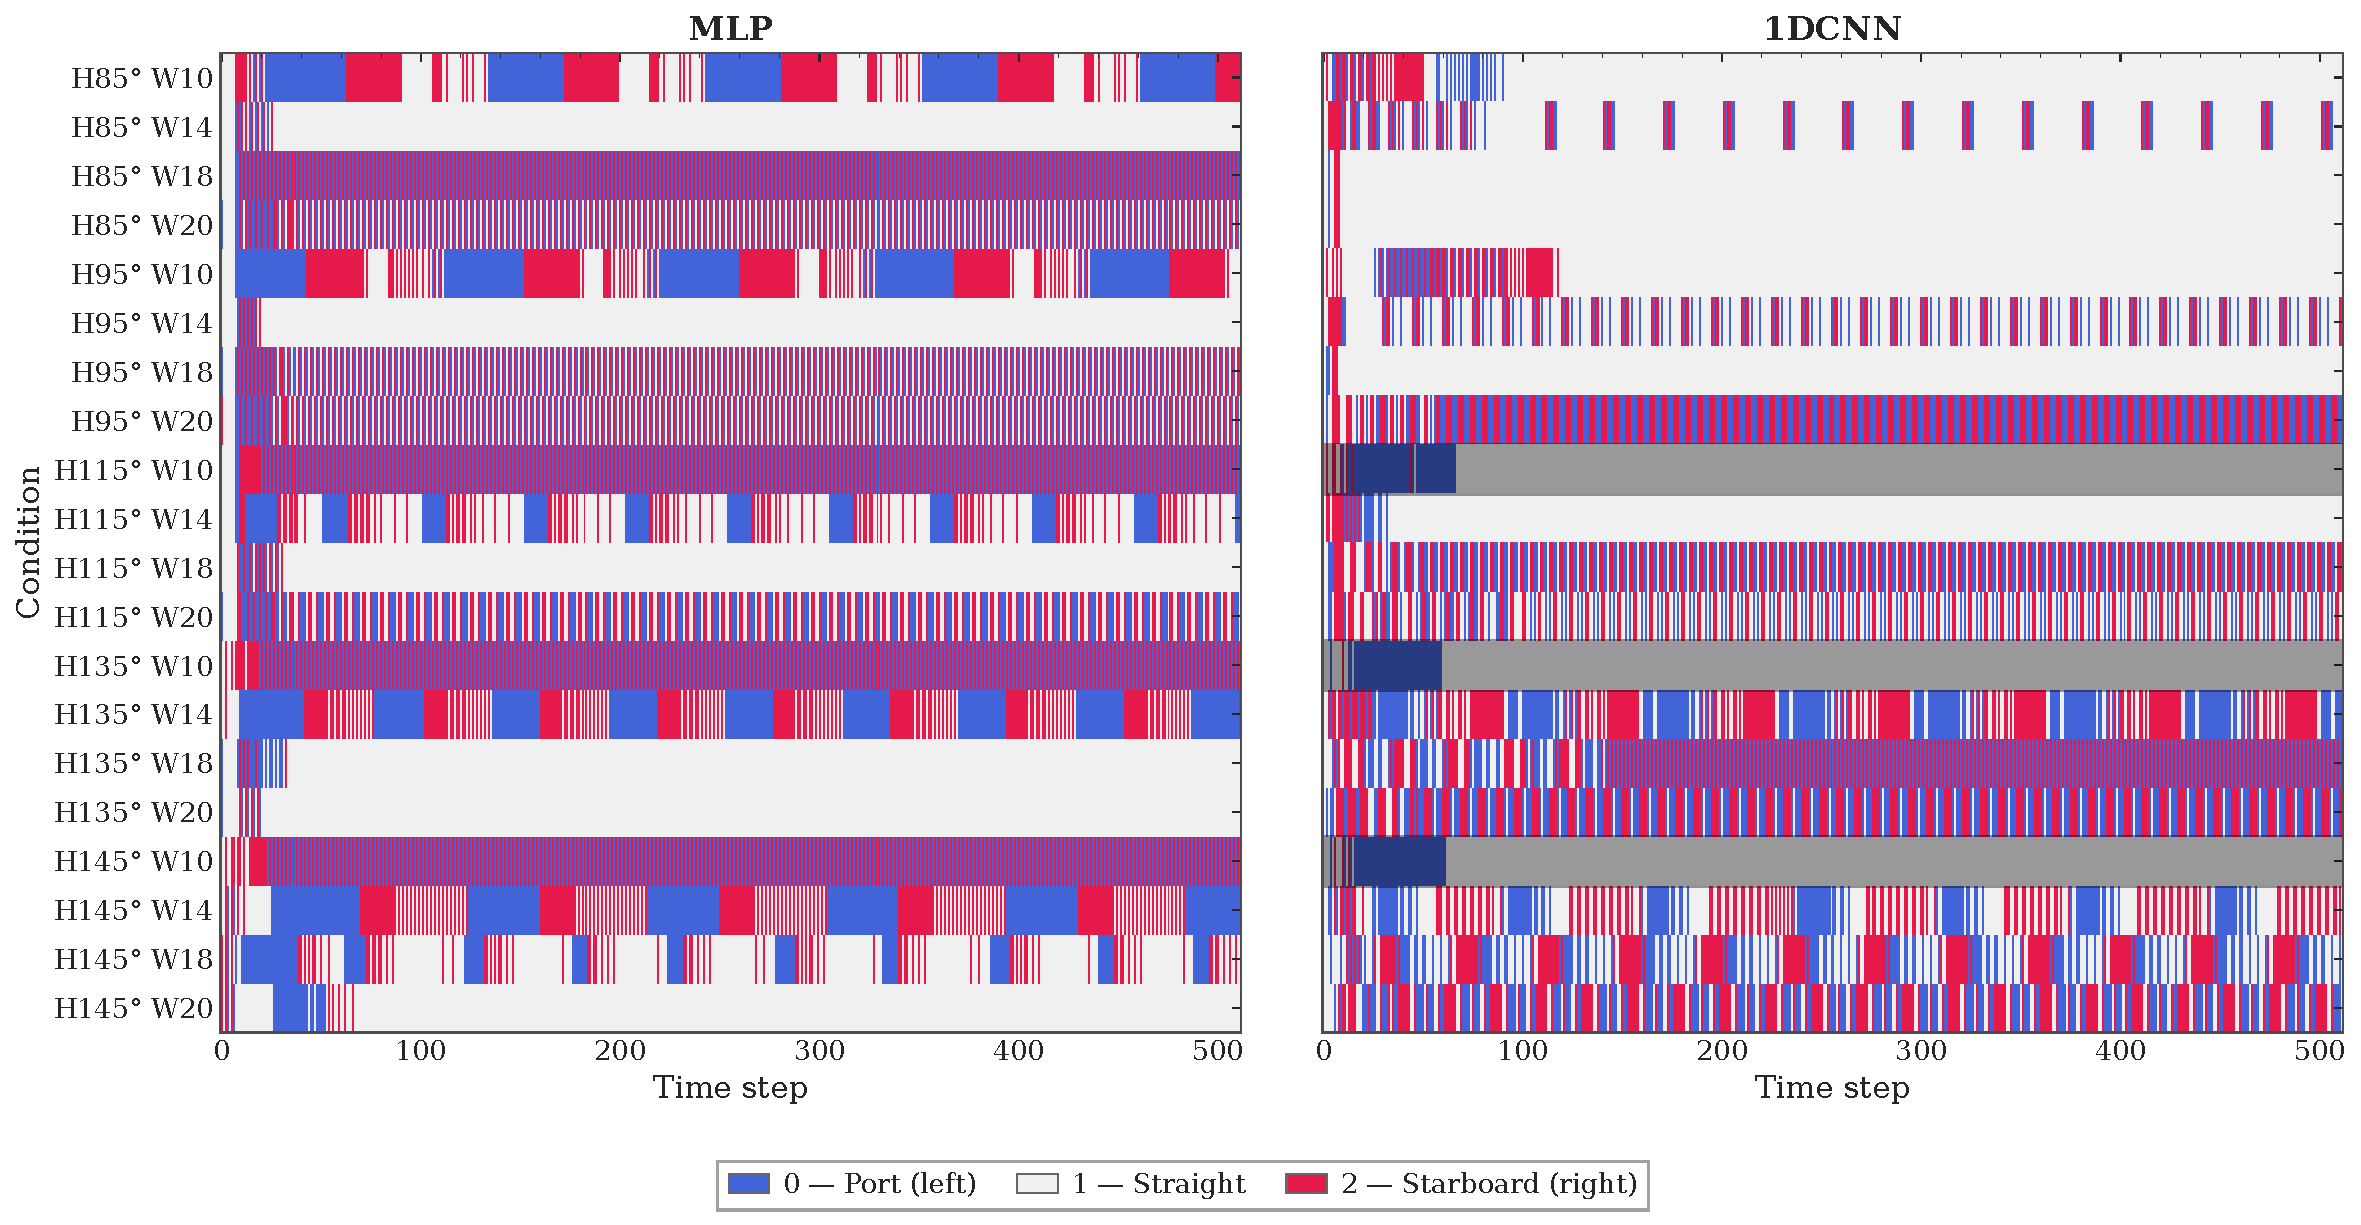
\includegraphics[width=1\linewidth]{resources/img/chapter4/action_heatmap_pub.pdf}
    \caption{Spatiotemporal heatmap of steering action offsets for MLP (left) and 1DCNN (right) across varying heading (H) and wind (W) conditions. The color gradient represents the difference between consecutive actions ($\Delta a_t = a_t - a_{t-1}$), where 0 (white) indicates a maintained course and 2 (dark red/blue) indicates maximum rudder deflection.}
    \label{fig:offsetmap}
\end{figure}

\justify To analyze the behavioral characteristics of the learned policies, we examine the action offset, defined as the numerical difference between the agent's current action and its previous action ($\Delta a_t = a_t - a_{t-1}$). This metric serves as a proxy for control \emph{jitter}: a high frequency of large offsets indicates aggressive or unstable steering behavior, whereas a concentration of small or zero offsets suggests smoother, more damped control resembling traditional PID-based steering. The command heatmaps in Figure~\ref{fig:offsetmap} reveal distinct operational signatures between the architectures across the 512-step evaluation episodes. The Multi-Layer Perceptron (MLP) exhibits pronounced policy instability, characterized by frequent high-magnitude offsets oscillating between port and starboard extremes. This ``chatter'' suggests that the MLP responds primarily to instantaneous environmental fluctuations without effectively leveraging temporal context, particularly near operational boundaries where maintaining stability becomes challenging.
\justify In contrast, the 1DCNN demonstrates a structured form of \emph{adaptive jitter}. Under high-wind conditions (14--20\,kts), steering corrections are concentrated around small-magnitude offsets, enabling the agent to maintain optimal foil lift and aerodynamic alignment while avoiding the large, energy-dissipating rudder oscillations observed in the MLP. However, this proactive control strategy introduces a trade-off in light-wind regimes (10\,kts). At headings H:115$^\circ$, H:135$^\circ$, and H:145$^\circ$, the 1DCNN's micro-correction behavior can lead to ``Out-of-Bounds'' (OOB) failures, as insufficient wind pressure limits the physical damping of steering inputs. These results indicate that while temporal feature extraction in the 1DCNN significantly enhances robustness and performance under high-load conditions, its aggressive optimization may reduce stability in marginal environments where the vessel operates near physical limits. This highlights a key design consideration for autonomous foiling controllers: balancing proactive performance optimization with fail-safe reactive mechanisms during low-energy operating states.


\subsection{Trajectory Analysis}
\begin{figure}[h]
    \centering
    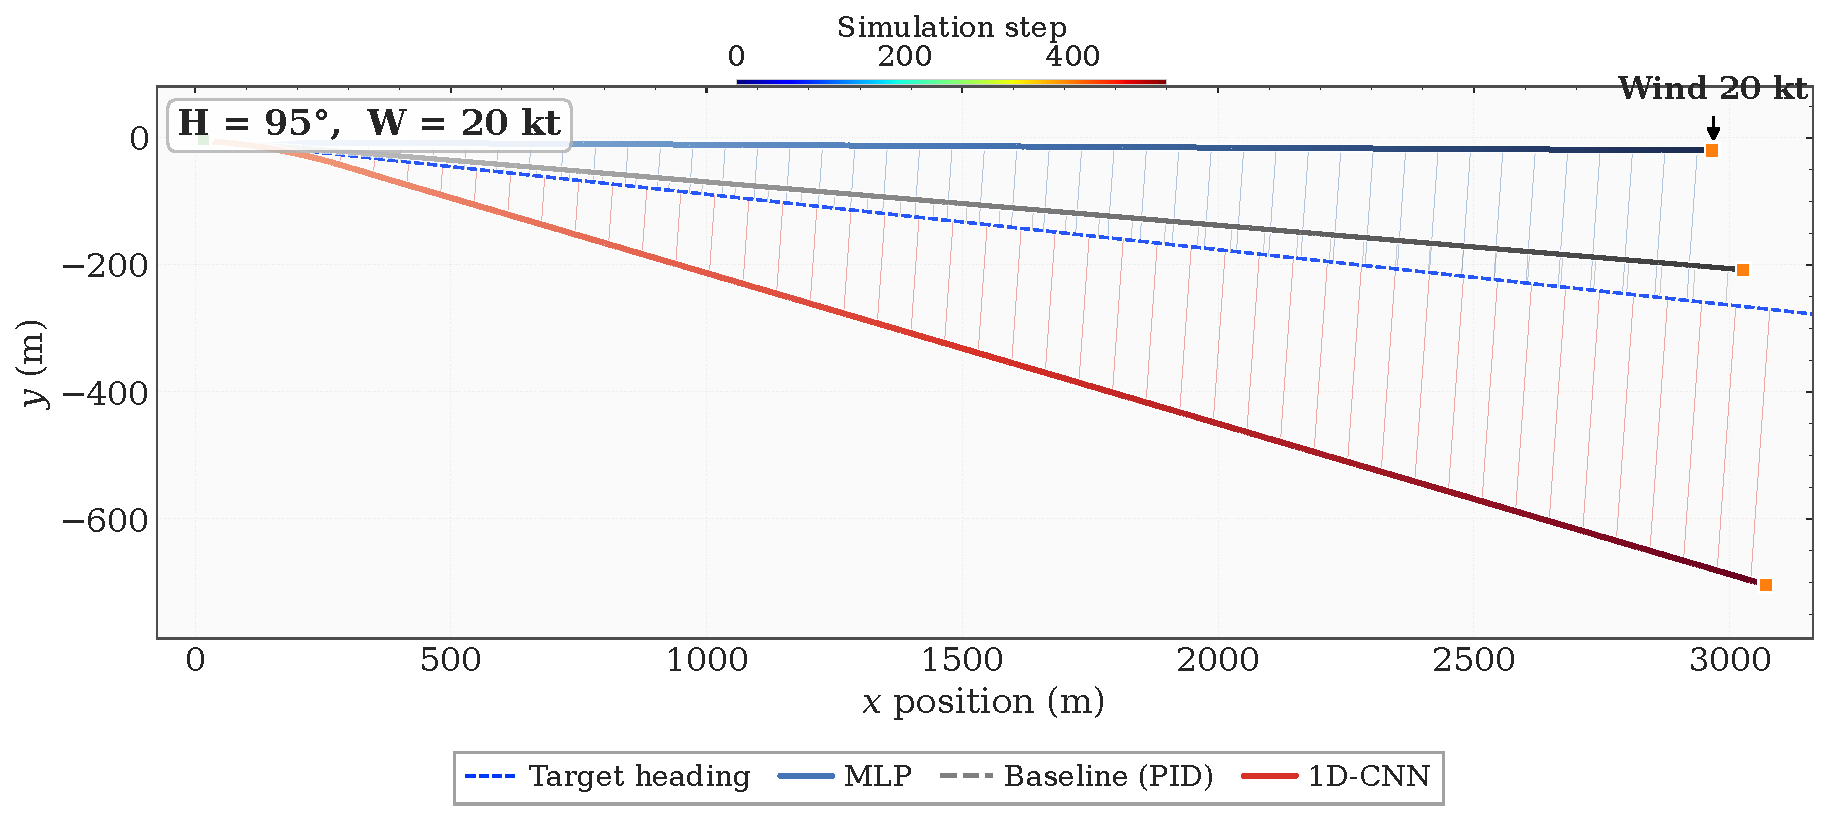
\includegraphics[width=0.9\linewidth]{resources/img/appendix/trajectory_samp.pdf}
    \caption{Distribution of action offsets ($\Delta a_t$) for MLP and 1DCNN across all test cases. The 1DCNN's distribution is more concentrated around zero, indicating smoother control, while the MLP exhibits a wider spread, reflecting higher jitter.}
    \label{fig:2dtrajectory}
\end{figure}

\justify The 2D trajectory plots (Figure~\ref{fig:2dtrajectory}) illustrate the spatial manifestations of the control policies discussed in the preceding sections. Under the boundary heading condition (H:85$^\circ$), the Baseline PID controller maintains a highly linear path but lacks proactive lift management, resulting in lower velocity and sub-optimal drift with the longest time-to-target. The MLP exhibits low-frequency oscillations in light-wind scenarios (W:10\,kt), producing a ``wavy'' trajectory that reflects the instability observed in the action-offset heatmaps, leading to increased drag and inefficient distance covered. In contrast, the 1DCNN demonstrates superior trajectory discipline, particularly under high-wind stress tests ($W{:}20\,\text{kt}$), maintaining the most direct and stable line toward the target by using ``adaptive jitter'' to make micro-adjustments and prevent the large-scale deviations seen in the MLP. While the 1DCNN can experience abrupt termination in low-wind edge cases due to OOB failures, its performance under viable foiling conditions remains the most robust and energy-efficient among the controllers.


\section{Conclusion and Future Work}
%These results indicate that while temporal feature extraction in the 1DCNN significantly enhances robustness and performance under high-load conditions, its aggressive optimization may reduce stability in marginal environments where the vessel operates near physical limits. This highlights a key design consideration for autonomous foiling controllers: balancing proactive performance optimization with fail-safe reactive mechanisms during low-energy operating states.

\paragraph{Conclusion}  This study shows that DRL provides a promising framework for the autopilot control of foiling sailboats compared to traditional PID-based systems. We successfully trained DRL agents capable of navigating stochastic upwind conditions ranging from 10 to 20\,knots. Our comparative analysis revealed that while the MLP remains a competitive reactive baseline, the state of the art 1DCNN architecture developed in this work emerged as the a promising robust solution for high performance regimes. 1DCNN achieves a peak steady-state CMG of 24.6\,knots. These results indicate that while temporal feature extraction in the 1DCNN significantly enhances robustness and performance under high-load conditions. Its adaptive jitter strategy effectively manages micro-corrections to maintain optimal foil lift, whereas the memoryless MLP often succumbs to inefficient oscillations or policy collapse under high wind loads. However, the identification of OOB failures in specific low wind edge cases suggests that aggressive performance optimization must be balanced with safe logic to ensure reliability across the entire polar range.

\paragraph{Future Work}  
Future work can focus on expanding the agent's operational envelope to cover a broader range of sailing conditions. To reduce the identified stability issues in marginal environments, we propose the integration of hierarchical RL structures, in which a high level 1DCNN oversees strategic performance while a low level reactive layer enforces safety constraints to prevent OOB excursions. Additionally, incorporating wave interactions and swell generation into the training environment will better prepare agents for the complex sea states. Finally, comparing the current 1DCNN architecture with recurrent models, such as Long Short-Term Memory (LSTM) networks, may provide insights into the most effective approach for capturing long-term temporal dependencies.


\section*{Acknowledgments}

We sincerely thank Camille and Benjamin Negrevergne from \href{https://nautia.fr/}{Nautia} for proposing this project and providing unwavering guidance throughout its development. Their support helped shape the work, ensured rigor, and gave us access to the \emph{BoatSimulator}, without which this project would not have been possible. We also thank the ENSAI for providing the computers to carry out the work which were essential for developing and testing our models.

\section*{Data Availability}
All data supporting the findings of this study, including training and evaluation scripts, are available at \url{https://github.com/Dilru1/deep-fooling}. A subset of derived data—including training checkpoints, \texttt{VecNormalize} statistics, and steady state CMG performance scores for both the MLP and 1DCNN architectures is also provided in the repository, along with the code used for data processing. Full evaluation datasets, high-resolution trajectory logs, and additional analysis files are available upon request. A web application for dynamically monitoring the RL agents is also accessible online. The state of the art \texttt{HistoryCNNExtractor} can be downloaded at \url{https://github.com/Dilru1/deep-fooling/blob/main/cnn_extractor.py}.



\vspace{1.5cm}
\begin{tcolorbox}[colback=blue!5!white, colframe=blue!40!black, arc=4pt, boxrule=0.8pt, left=10pt, right=10pt, top=10pt, bottom=10pt]
\begin{center}
\textit{
``The pessimist complains about the wind; the optimist expects it to change; the realist adjusts the sails.''\\
--- William Arthur Ward
}

\vspace{0.5cm}

\textit{
In the context of RL, the agent reflects the realist. It does not assume a favorable environment nor resist uncertainty, but instead learns a policy that continuously adapts to changing conditions. Through iterative interaction, feedback, and optimization, intelligent control emerges not from predicting the future perfectly, but from learning how to adjust the sails at every moment.}
\end{center}
\end{tcolorbox}       
%\input{chapters/chapter6}
%\newpage

%\bibliographystyle{plain}
%\bibliography{ref}

\appendix
\section{Complete Experimental Results Table}
\label{sec:vmg}

\begin{table}[H]
\centering
\footnotesize
\setlength{\tabcolsep}{3.5pt}
\renewcommand{\arraystretch}{0.88}
\begin{tabular}{@{}rr rrr rrr rrr@{}}
\toprule
& & \multicolumn{3}{c}{\textbf{MLP}} & \multicolumn{3}{c}{\textbf{PID}} & \multicolumn{3}{c}{\textbf{1DCNN (This work)}} \\
\cmidrule(lr){3-5} \cmidrule(lr){6-8} \cmidrule(lr){9-11}
Hdg ($^\circ$) & Wind (kt) & CMG & Err ($^\circ$) & XTE (m) & CMG & Err ($^\circ$) & XTE (m) & CMG & Err ($^\circ$) & XTE (m) \\
\midrule
85  & 10 &  9.44 & 10.40 & 155.12 & 10.95 & 1.25 & 21.31 & \textcolor{red}{11.53} &  6.10 & 108.46 \\
85  & 14 & 16.67 &  0.60 &  15.41 & 16.51 & 1.54 & 39.66 & \textcolor{red}{17.23} &  3.75 & 100.85 \\
85  & 18 & 19.35 &  2.39 &  72.49 & 19.62 & 0.94 & 28.84 & \textcolor{red}{19.99} &  0.99 &  30.94 \\
85  & 20 & 22.19 &  4.65 & 162.10 & 23.11 & 1.05 & 38.08 & \textcolor{red}{23.50} &  0.88 &  32.36 \\
\midrule
95  & 10 &  9.49 & 11.90 & 179.37 & 11.00 & 1.32 & 22.67 & \textcolor{red}{11.04} & 15.58 & 283.57 \\
95  & 14 & 16.59 &  0.62 &  15.95 & 16.48 & 1.55 & 39.78 & \textcolor{red}{17.02} &  3.95 & 105.38 \\
95  & 18 & 20.35 &  1.70 &  54.21 & 20.40 & 0.97 & 30.99 & \textcolor{red}{20.54} &  0.02 &   0.58 \\
95  & 20 & 23.24 &  4.61 & 168.55 & 23.87 & 1.10 & 40.94 & \textcolor{red}{24.59} &  7.71 & 299.62 \\
\midrule
115 & 10 & \textcolor{red}{10.14} &  6.57 & 104.95 &  9.94 & 1.47 & 22.78 & N/A   & N/A   & N/A    \\
115 & 14 & 14.00 & 11.88 & 266.68 & \textcolor{red}{15.05} & 1.54 & 36.16 & 14.98 &  2.01 &  48.00 \\
115 & 18 & 20.42 &  2.07 &  66.18 & 20.50 & 1.08 & 34.57 & \textcolor{red}{20.53} &  7.10 & 230.81 \\
115 & 20 & 24.00 &  5.56 & 209.87 & \textcolor{red}{24.36} & 1.18 & 44.99 & 23.99 &  7.92 & 302.95 \\
\midrule
135 & 10 &  8.39 & 10.32 & 137.14 & \textcolor{red}{8.71} & 1.64 & 22.26 & N/A   & N/A   & N/A    \\
135 & 14 & 11.49 & 19.33 & 363.91 & \textcolor{red}{12.83} & 1.61 & 32.11 & 12.53 &  0.41 &   7.74 \\
135 & 18 & 17.05 & 11.39 & 309.64 & 17.64 & 1.06 & 29.34 & \textcolor{red}{17.65} &  0.15 &   3.38 \\
135 & 20 & \textcolor{red}{19.77} &  2.07 &  63.96 & 19.76 & 1.08 & 33.37 & 19.39 &  4.49 & 137.72 \\
\midrule
145 & 10 &  6.95 & 11.90 & 132.60 & \textcolor{red}{8.23} & 1.76 & 22.41 & N/A   & N/A   & N/A    \\
145 & 14 &  9.89 & 22.01 & 360.30 & \textcolor{red}{11.81} & 1.69 & 30.97 & 11.56 &  7.62 & 138.39 \\
145 & 18 & 13.49 & 23.97 & 546.05 & \textcolor{red}{15.85} & 1.13 & 27.78 & 15.84 &  2.86 &  70.94 \\
145 & 20 & 15.66 & 18.04 & 463.74 & \textcolor{red}{17.55} & 1.08 & 29.46 & 17.47 &  0.20 &   5.49 \\
\bottomrule
\end{tabular}
\caption{Systematic comparison of navigational metrics across architectural groups, sorted by heading and wind intensity.}
\label{tab:results_sorted}
\end{table}

\section{CMG Improvement Over Baseline}
\label{sec:cmg_improvement}

\begin{table}[htbp]
\centering
\footnotesize
\setlength{\tabcolsep}{5pt}
\renewcommand{\arraystretch}{0.92}
\begin{tabular}{@{}rr rrr rr@{}}
\toprule
& & \multicolumn{3}{c}{\textbf{CMG Values}} & \multicolumn{2}{c}{\textbf{\% Improvement vs PID}} \\
\cmidrule(lr){3-5} \cmidrule(lr){6-7}
Hdg ($^\circ$) & Wind (kt) & MLP & PID & 1DCNN & MLP & 1DCNN \\
\midrule
85  & 10 &  9.44 & 10.95 & 11.53 & $-13.77$ & \textcolor{red}{$+5.27$} \\
85  & 14 & 16.67 & 16.51 & 17.23 & \textcolor{red}{$+0.92$}  & \textcolor{red}{$+4.33$} \\
85  & 18 & 19.35 & 19.62 & 19.99 & $-1.36$  & \textcolor{red}{$+1.90$} \\
85  & 20 & 22.19 & 23.11 & 23.50 & $-3.95$  & \textcolor{red}{$+1.72$} \\
\midrule
95  & 10 &  9.49 & 11.00 & 11.04 & $-13.71$ & \textcolor{red}{$+0.36$} \\
95  & 14 & 16.59 & 16.48 & 17.02 & \textcolor{red}{$+0.71$}  & \textcolor{red}{$+3.28$} \\
95  & 18 & 20.35 & 20.40 & 20.54 & $-0.28$  & \textcolor{red}{$+0.67$} \\
95  & 20 & 23.24 & 23.87 & 24.59 & $-2.61$  & \textcolor{red}{$+3.02$} \\
\midrule
115 & 10 & 10.14 &  9.94 & N/A  & \textcolor{red}{$+2.03$} & N/A     \\
115 & 14 & 14.00 & 15.05 & 14.98 & $-6.98$  & $-0.44$  \\
115 & 18 & 20.42 & 20.50 & 20.53 & $-0.39$  & \textcolor{red}{$+0.14$} \\
115 & 20 & 24.00 & 24.36 & 23.99 & $-1.45$  & $-1.48$  \\
\midrule
135 & 10 &  8.39 &  8.71 & N/A  & $-3.73$  & N/A     \\
135 & 14 & 11.49 & 12.83 & 12.53 & $-10.47$ & $-2.35$  \\
135 & 18 & 17.05 & 17.64 & 17.65 & $-3.36$  & \textcolor{red}{$+0.06$} \\
135 & 20 & 19.77 & 19.76 & 19.39 & \textcolor{red}{$+0.07$} & $-1.87$  \\
\midrule
145 & 10 &  6.95 &  8.23 & N/A  & $-15.55$ & N/A     \\
145 & 14 &  9.89 & 11.81 & 11.56 & $-16.25$ & $-2.15$  \\
145 & 18 & 13.49 & 15.85 & 15.84 & $-14.89$ & $-0.07$  \\
145 & 20 & 15.66 & 17.55 & 17.47 & $-10.78$ & $-0.44$  \\
%\midrule
%\multicolumn{5}{@{}r}{\textbf{Average}} & $\mathbf{-5.80}$ & $\mathbf{+0.70}$ \\
%\multicolumn{5}{@{}r}{\textbf{Rows beating PID}} & $\mathbf{3/17}$ & $\mathbf{10/17}$ \\
\bottomrule
\end{tabular}
\caption{Percentage CMG improvement of MLP and 1DCNN over the PID baseline. N/A indicates the model failed for that condition. Positive values (red) indicate the model outperforms PID.}
\label{tab:cmg_improvement}
\end{table}



\section{Complete Trajectory Comparison}
\label{sec:cmg_improvement}

\begin{figure}[H]
    \centering
    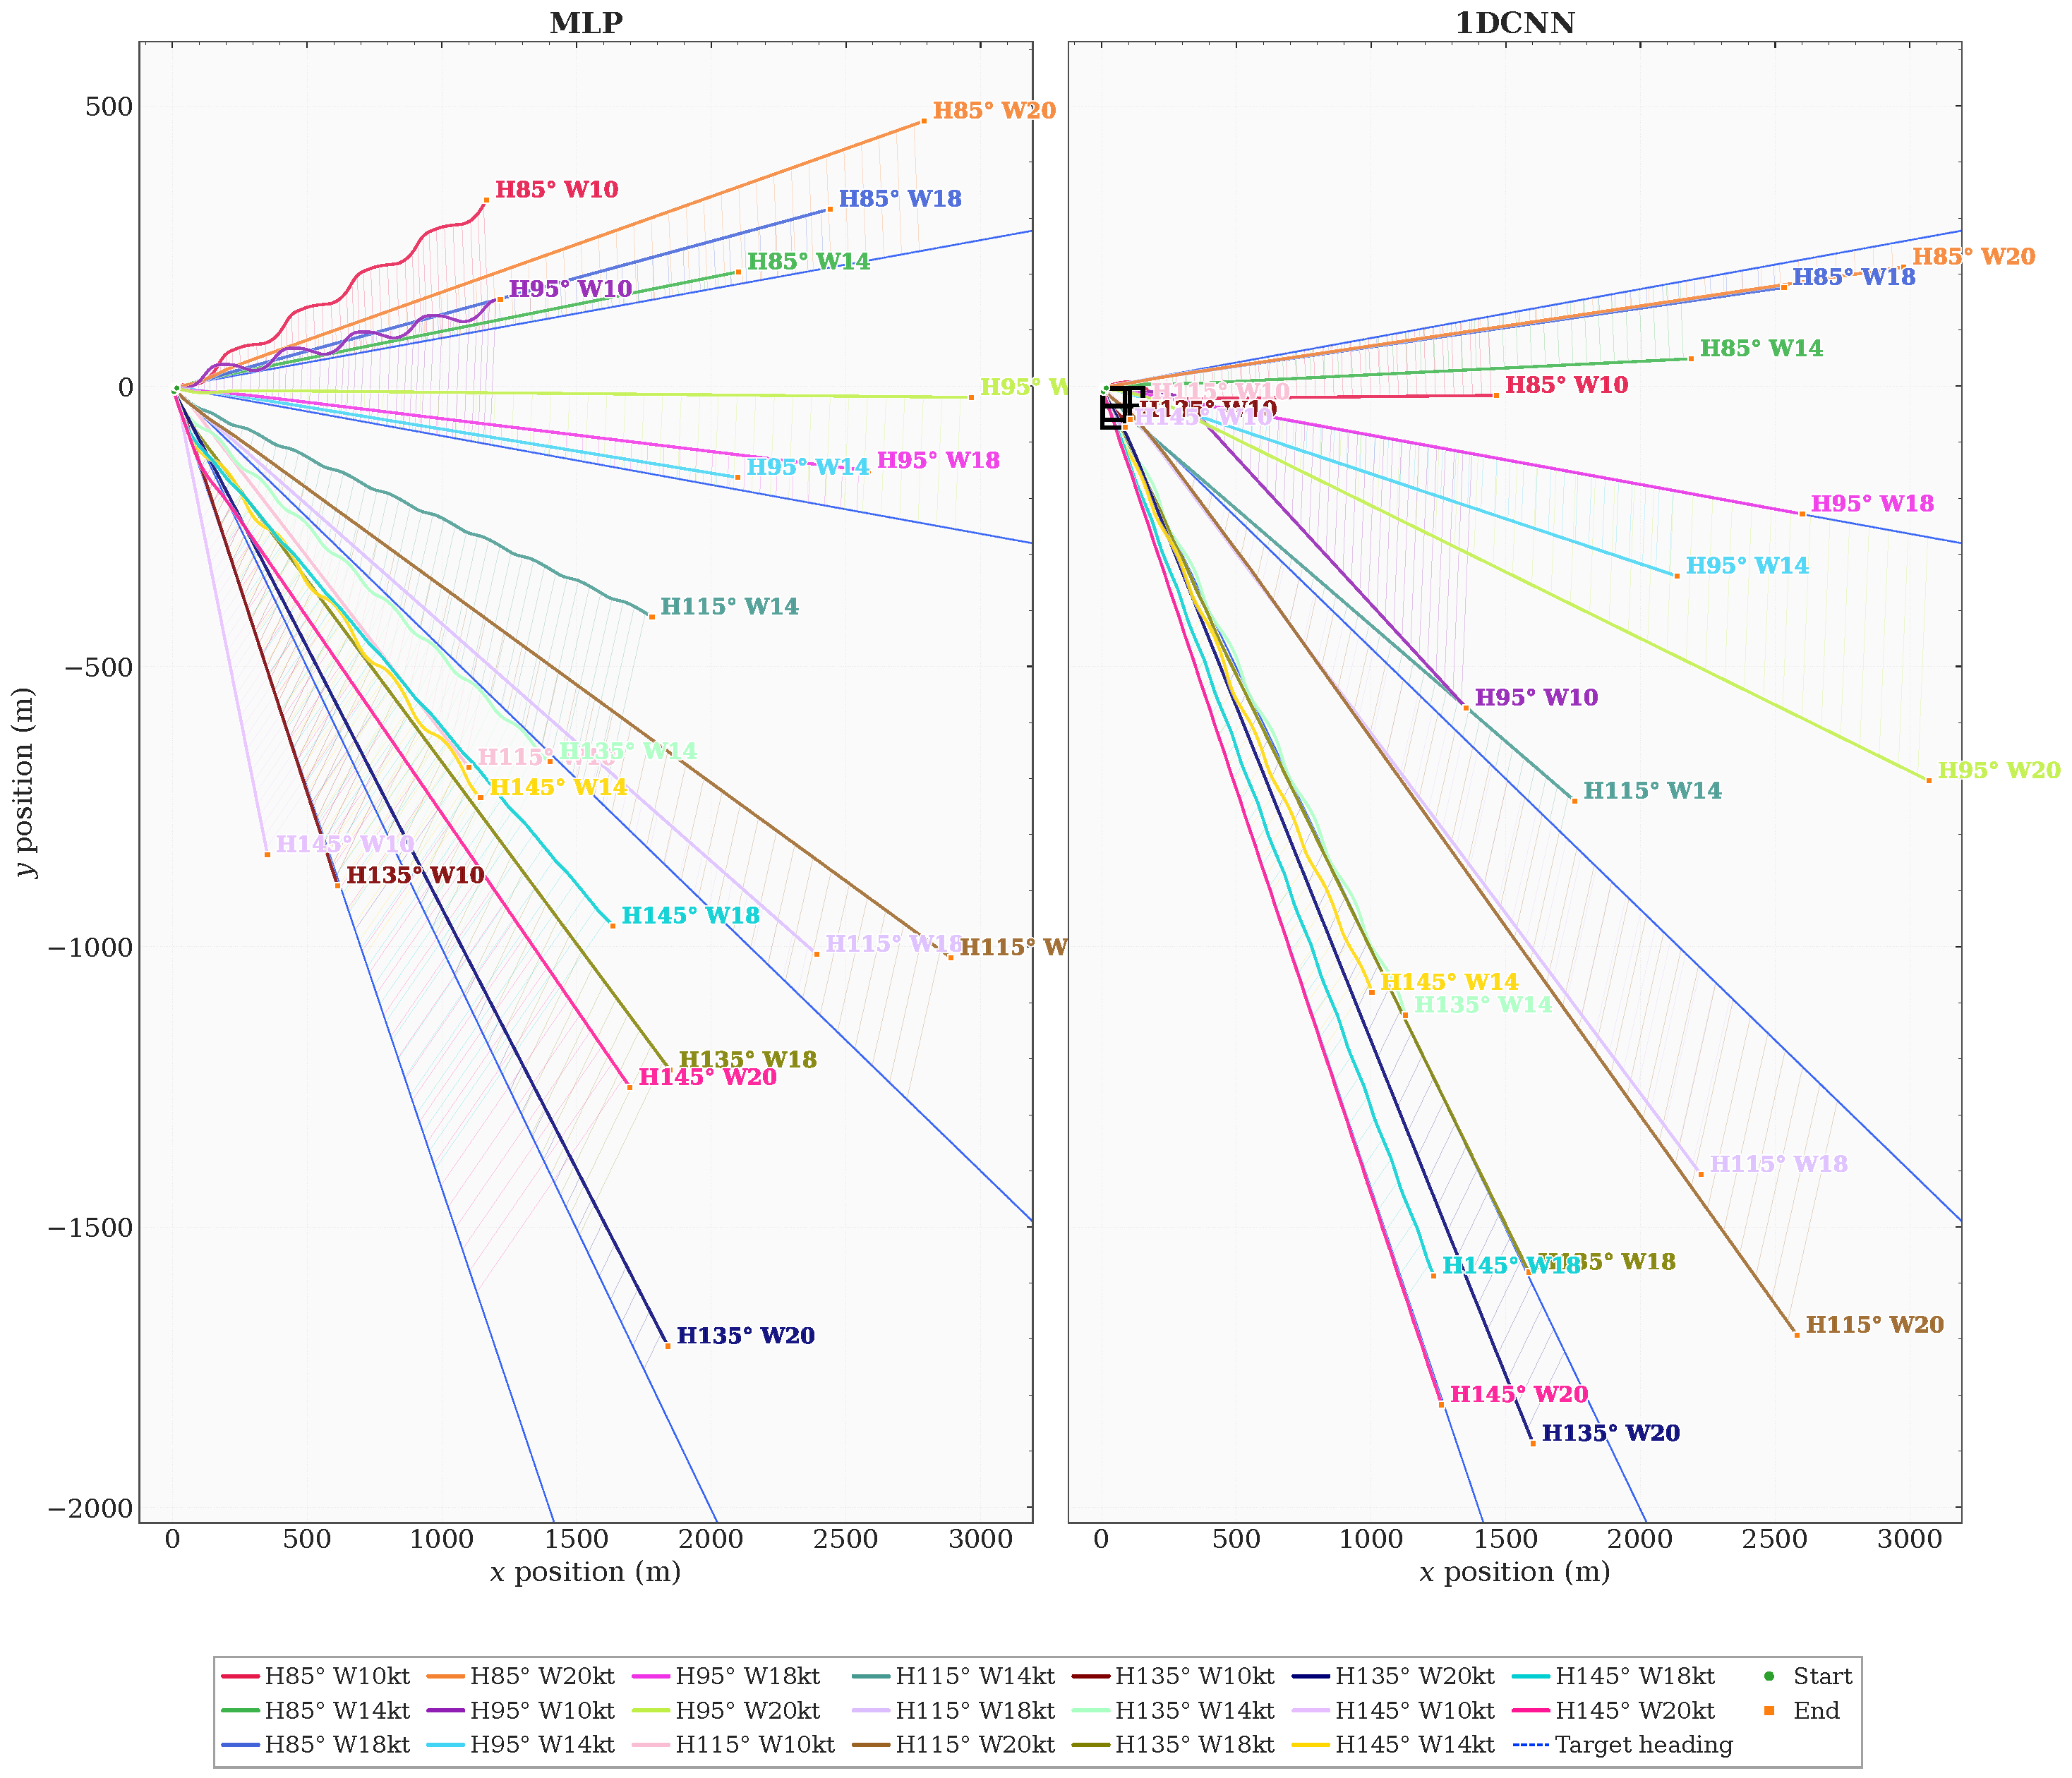
\includegraphics[width=0.8\linewidth]{resources/img/appendix/trajectory_grid_pub.pdf}
    \caption{Trajectory comparison across both architectures under all heading and wind conditions.}
    \label{fig:trajectory_grid}
\end{figure}

\justify
The trajectory plots provide a qualitative comparison of steering behaviors across the evaluation grid. The Baseline controller produces smooth, linear paths but exhibits significant drift under high-wind conditions, indicating limited proactive adaptation. The MLP shows clear instability, particularly at $H:85^\circ \mid W:10\,\text{kt}$, where large oscillations suggest poor damping and reduced navigational efficiency. In contrast, the 1DCNN maintains the most robust trajectories, adhering closely to the intended path even under 20\,kt stress tests. A notable exception arises in light-wind conditions (10\,kt) at headings of $115^\circ$, $135^\circ$, and $145^\circ$, where aggressive micro-corrections occasionally lead to ``Out-of-Bound'' (OOB) terminations. Despite these edge-case failures, the 1DCNN consistently outperforms the other architectures in high-performance foiling scenarios.





\end{document}